\documentclass[12pt]{article}
\usepackage{combelow}
\usepackage{amsmath,amssymb,amsthm}
\usepackage{graphicx}
\usepackage{tikz}
\usepackage{booktabs}
\usepackage{array}
\usepackage[shortlabels]{enumitem}
\setlength{\emergencystretch}{2em}
\usepackage[colorlinks=true,linkcolor=blue!45!black,citecolor=blue!45!black,urlcolor=blue!45!black]{hyperref}
\hypersetup{pdftitle={Maximum Blackouts That Keep Every Lattice Rectangle Identifiable},pdfauthor={Arjun Pemmasani}}

\definecolor{kgray}{HTML}{AAAAAA}
\definecolor{kyellow}{HTML}{FFF64C}
\definecolor{kred}{HTML}{FF6666}
\tikzset{
  lab/.style={font=\scriptsize,text=black!55},
  capt/.style={font=\small},
}

\theoremstyle{plain}
\newtheorem{theorem}{Theorem}
\newtheorem{lemma}[theorem]{Lemma}
\newtheorem{proposition}[theorem]{Proposition}
\newtheorem{corollary}[theorem]{Corollary}
\newtheorem{introthm}{Theorem}
\renewcommand{\theintrothm}{\Alph{introthm}}
\theoremstyle{definition}
\newtheorem{definition}[theorem]{Definition}
\theoremstyle{remark}
\newtheorem{remark}[theorem]{Remark}

\newcommand{\seqnum}[1]{\href{https://oeis.org/#1}{\rm \underline{#1}}}
\newcommand{\pres}{P_S}
\newcommand{\kA}{\mathsf{A}}
\newcommand{\kB}{\mathsf{B}}
\newcommand{\kC}{\mathsf{C}}
\newcommand{\kE}{\mathsf{E}}

\title{Maximum Blackouts That Keep Every Lattice Rectangle Identifiable}
\author{Arjun Pemmasani\\
Department of Mathematics\\
Harvey Mudd College\\
Claremont, CA 91711\\
USA\\
\texttt{apemmasani@hmc.edu}}
\date{}

\begin{document}
\maketitle

\begin{abstract}
Kagey's Problem 001 concerns a grid of points, some of them blacked out. A rectangle
with its corners on grid points, tilted or not, shows only its white corners. We ask how
many points can be blacked out while every rectangle stays determined by what it shows.
We study the maximum blackout and the number of optima, tabulated in A397315 and A399580
of the On-Line Encyclopedia of Integer Sequences. A row-column graph and Mantel's theorem
bound the maximum by the width plus a quarter of the squared height. We find the maximum
on up to five rows at every width, and on six rows from width 15 on. The five-row result
refutes our earlier guess that the maximum is the sum of the two sides. We count the three-row optima exactly and
find the growth rate on four rows. At every fixed height, the maximum minus the width is
eventually periodic, and the optimum counts have a rational generating function. Some
values rest on computer checks.
\end{abstract}

\section{Introduction}\label{sec:intro}

Start with an $h\times m$ grid and black out some of its points.
The game master chooses a rectangle (tilted ones are allowed) and tells
you which of its corners are white. Can you recover all four corners?
Kagey~\cite{kageyG4G14,kagey001} asks how many points can be blacked out
while keeping the answer unique for every rectangle.
Such a set is a \emph{valid blackout} (Definition~\ref{def:valid}).
One round is shown in Figure~\ref{fig:game}.

\begin{figure}[t]
\centering
\resizebox{\textwidth}{!}{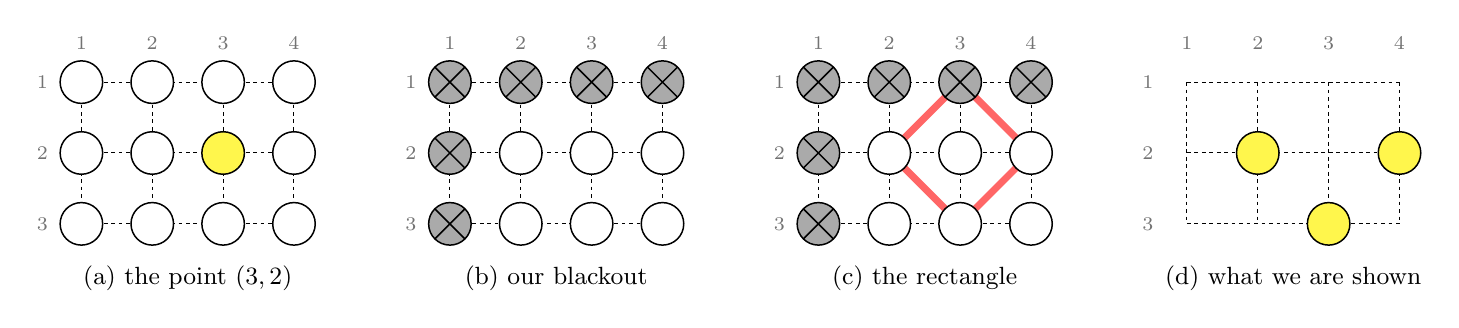
\begin{tikzpicture}[x=0.9cm,y=0.9cm,baseline=(current bounding box.north)]
  \begin{scope}[xshift=0.000cm]
    \draw[black,line width=0.36pt,dash pattern=on 1.35pt off 1.35pt] (1,-1) -- (4,-1) (1,-2) -- (4,-2) (1,-3) -- (4,-3) (1,-1) -- (1,-3) (2,-1) -- (2,-3) (3,-1) -- (3,-3) (4,-1) -- (4,-3);
    \filldraw[fill=white,draw=black,line width=0.54pt] (1,-1) circle (0.3);
    \filldraw[fill=white,draw=black,line width=0.54pt] (2,-1) circle (0.3);
    \filldraw[fill=white,draw=black,line width=0.54pt] (3,-1) circle (0.3);
    \filldraw[fill=white,draw=black,line width=0.54pt] (4,-1) circle (0.3);
    \filldraw[fill=white,draw=black,line width=0.54pt] (1,-2) circle (0.3);
    \filldraw[fill=white,draw=black,line width=0.54pt] (2,-2) circle (0.3);
    \filldraw[fill=kyellow,draw=black,line width=0.54pt] (3,-2) circle (0.3);
    \filldraw[fill=white,draw=black,line width=0.54pt] (4,-2) circle (0.3);
    \filldraw[fill=white,draw=black,line width=0.54pt] (1,-3) circle (0.3);
    \filldraw[fill=white,draw=black,line width=0.54pt] (2,-3) circle (0.3);
    \filldraw[fill=white,draw=black,line width=0.54pt] (3,-3) circle (0.3);
    \filldraw[fill=white,draw=black,line width=0.54pt] (4,-3) circle (0.3);
    \node[lab] at (1,-0.45) {1};
    \node[lab] at (2,-0.45) {2};
    \node[lab] at (3,-0.45) {3};
    \node[lab] at (4,-0.45) {4};
    \node[lab] at (0.45,-1) {1};
    \node[lab] at (0.45,-2) {2};
    \node[lab] at (0.45,-3) {3};
    \node[capt,anchor=north] at (2.50,-3.45) {(a) the point $(3,2)$};
  \end{scope}
  \begin{scope}[xshift=4.680cm]
    \draw[black,line width=0.36pt,dash pattern=on 1.35pt off 1.35pt] (1,-1) -- (4,-1) (1,-2) -- (4,-2) (1,-3) -- (4,-3) (1,-1) -- (1,-3) (2,-1) -- (2,-3) (3,-1) -- (3,-3) (4,-1) -- (4,-3);
    \filldraw[fill=kgray,draw=black,line width=0.54pt] (1,-1) circle (0.3);
    \draw[black,line width=0.54pt] (0.788,-0.788) -- (1.212,-1.212) (0.788,-1.212) -- (1.212,-0.788);
    \filldraw[fill=kgray,draw=black,line width=0.54pt] (2,-1) circle (0.3);
    \draw[black,line width=0.54pt] (1.788,-0.788) -- (2.212,-1.212) (1.788,-1.212) -- (2.212,-0.788);
    \filldraw[fill=kgray,draw=black,line width=0.54pt] (3,-1) circle (0.3);
    \draw[black,line width=0.54pt] (2.788,-0.788) -- (3.212,-1.212) (2.788,-1.212) -- (3.212,-0.788);
    \filldraw[fill=kgray,draw=black,line width=0.54pt] (4,-1) circle (0.3);
    \draw[black,line width=0.54pt] (3.788,-0.788) -- (4.212,-1.212) (3.788,-1.212) -- (4.212,-0.788);
    \filldraw[fill=kgray,draw=black,line width=0.54pt] (1,-2) circle (0.3);
    \draw[black,line width=0.54pt] (0.788,-1.788) -- (1.212,-2.212) (0.788,-2.212) -- (1.212,-1.788);
    \filldraw[fill=white,draw=black,line width=0.54pt] (2,-2) circle (0.3);
    \filldraw[fill=white,draw=black,line width=0.54pt] (3,-2) circle (0.3);
    \filldraw[fill=white,draw=black,line width=0.54pt] (4,-2) circle (0.3);
    \filldraw[fill=kgray,draw=black,line width=0.54pt] (1,-3) circle (0.3);
    \draw[black,line width=0.54pt] (0.788,-2.788) -- (1.212,-3.212) (0.788,-3.212) -- (1.212,-2.788);
    \filldraw[fill=white,draw=black,line width=0.54pt] (2,-3) circle (0.3);
    \filldraw[fill=white,draw=black,line width=0.54pt] (3,-3) circle (0.3);
    \filldraw[fill=white,draw=black,line width=0.54pt] (4,-3) circle (0.3);
    \node[lab] at (1,-0.45) {1};
    \node[lab] at (2,-0.45) {2};
    \node[lab] at (3,-0.45) {3};
    \node[lab] at (4,-0.45) {4};
    \node[lab] at (0.45,-1) {1};
    \node[lab] at (0.45,-2) {2};
    \node[lab] at (0.45,-3) {3};
    \node[capt,anchor=north] at (2.50,-3.45) {(b) our blackout};
  \end{scope}
  \begin{scope}[xshift=9.360cm]
    \draw[black,line width=0.36pt,dash pattern=on 1.35pt off 1.35pt] (1,-1) -- (4,-1) (1,-2) -- (4,-2) (1,-3) -- (4,-3) (1,-1) -- (1,-3) (2,-1) -- (2,-3) (3,-1) -- (3,-3) (4,-1) -- (4,-3);
    \draw[kred,line width=2.55pt,line join=round] (2,-2) -- (3,-1) -- (4,-2) -- (3,-3) -- cycle;
    \filldraw[fill=kgray,draw=black,line width=0.54pt] (1,-1) circle (0.3);
    \draw[black,line width=0.54pt] (0.788,-0.788) -- (1.212,-1.212) (0.788,-1.212) -- (1.212,-0.788);
    \filldraw[fill=kgray,draw=black,line width=0.54pt] (2,-1) circle (0.3);
    \draw[black,line width=0.54pt] (1.788,-0.788) -- (2.212,-1.212) (1.788,-1.212) -- (2.212,-0.788);
    \filldraw[fill=kgray,draw=black,line width=0.54pt] (3,-1) circle (0.3);
    \draw[black,line width=0.54pt] (2.788,-0.788) -- (3.212,-1.212) (2.788,-1.212) -- (3.212,-0.788);
    \filldraw[fill=kgray,draw=black,line width=0.54pt] (4,-1) circle (0.3);
    \draw[black,line width=0.54pt] (3.788,-0.788) -- (4.212,-1.212) (3.788,-1.212) -- (4.212,-0.788);
    \filldraw[fill=kgray,draw=black,line width=0.54pt] (1,-2) circle (0.3);
    \draw[black,line width=0.54pt] (0.788,-1.788) -- (1.212,-2.212) (0.788,-2.212) -- (1.212,-1.788);
    \filldraw[fill=white,draw=black,line width=0.54pt] (2,-2) circle (0.3);
    \filldraw[fill=white,draw=black,line width=0.54pt] (3,-2) circle (0.3);
    \filldraw[fill=white,draw=black,line width=0.54pt] (4,-2) circle (0.3);
    \filldraw[fill=kgray,draw=black,line width=0.54pt] (1,-3) circle (0.3);
    \draw[black,line width=0.54pt] (0.788,-2.788) -- (1.212,-3.212) (0.788,-3.212) -- (1.212,-2.788);
    \filldraw[fill=white,draw=black,line width=0.54pt] (2,-3) circle (0.3);
    \filldraw[fill=white,draw=black,line width=0.54pt] (3,-3) circle (0.3);
    \filldraw[fill=white,draw=black,line width=0.54pt] (4,-3) circle (0.3);
    \node[lab] at (1,-0.45) {1};
    \node[lab] at (2,-0.45) {2};
    \node[lab] at (3,-0.45) {3};
    \node[lab] at (4,-0.45) {4};
    \node[lab] at (0.45,-1) {1};
    \node[lab] at (0.45,-2) {2};
    \node[lab] at (0.45,-3) {3};
    \node[capt,anchor=north] at (2.50,-3.45) {(c) the rectangle};
  \end{scope}
  \begin{scope}[xshift=14.040cm]
    \draw[black,line width=0.36pt,dash pattern=on 1.35pt off 1.35pt] (1,-1) -- (4,-1) (1,-2) -- (4,-2) (1,-3) -- (4,-3) (1,-1) -- (1,-3) (2,-1) -- (2,-3) (3,-1) -- (3,-3) (4,-1) -- (4,-3);
    \filldraw[fill=kyellow,draw=black,line width=0.54pt] (2,-2) circle (0.3);
    \filldraw[fill=kyellow,draw=black,line width=0.54pt] (4,-2) circle (0.3);
    \filldraw[fill=kyellow,draw=black,line width=0.54pt] (3,-3) circle (0.3);
    \node[lab] at (1,-0.45) {1};
    \node[lab] at (2,-0.45) {2};
    \node[lab] at (3,-0.45) {3};
    \node[lab] at (4,-0.45) {4};
    \node[lab] at (0.45,-1) {1};
    \node[lab] at (0.45,-2) {2};
    \node[lab] at (0.45,-3) {3};
    \node[capt,anchor=north] at (2.50,-3.45) {(d) what we are shown};
  \end{scope}
\end{tikzpicture}}
\caption{One round on a largest valid blackout of the $3\times4$ grid
(Section~\ref{sec:three}). Points are (column, row). Gray crossed circles are black. Panel (c) shows the red
rectangle, and (d) its yellow corners. The three yellow corners fix the fourth by
Lemma~\ref{lem:threecorners}.}
\label{fig:game}
\end{figure}

Write $f(h,m)$ for the most points we can black out, and $a_h(m)$
for the number of ways to attain it. The conjectures recorded in our
OEIS entries \seqnum{A397315} and \seqnum{A399580}~\cite{oeis} were
$f(3,m)=m+2$ and $f(h,m)=h+m$ for $\min(h,m)\ge4$, with exceptions
$f(4,4)=7$ and $f(4,5)=8$. The first was proved in Lean by the Omega
Institute, whose pull request was merged on 15 September
2026~\cite{trureturing2026}. Our independent proof combines the row
bound (Theorem~\ref{thm:rowbound}) and the boundary cross
(Lemma~\ref{lem:cross}). The second guess breaks at $5\times8$
(Theorem~\ref{thm:fiverow}). Throughout, put $q_h=\lfloor h^2/4\rfloor$.
Computer-assisted claims are marked, with evidence in
Table~\ref{tab:evidence}.

The main results follow, with proof locations in parentheses.

\begin{introthm}[narrow grids]\label{thm:A}
\leavevmode
\begin{enumerate}[(a)]
\item We have $f(h,m)\ge h+m-1$, and $f(h,m)\le m+q_h$ if $m\ge3$. \textup{(Lemma~\ref{lem:cross}
and Theorem~\ref{thm:rowbound}, Section~\ref{sec:graph}.)}
\item We have $f(2,m)=m+1$ and $f(3,m)=m+2$ for $m\ge3$, $f(4,m)=m+4$ for $m\ge6$,
and $f(5,5)=10$. \textup{(Theorem~\ref{thm:strip}, Section~\ref{sec:three},
Theorem~\ref{thm:fourvalue}, and Theorem~\ref{thm:fivefive}(a).)}
\item (Computer-assisted, with checked certificates for $f(5,6)$ and $f(5,7)$, and the last
claim checked in Lean.) We have $f(4,4)=7$, $f(4,5)=8$,
$f(5,6)=11$, $f(5,7)=12$, and $f(5,m)=m+6$ for $m\ge8$. \textup{(Corollary~\ref{cor:fourboundary}
and Theorem~\ref{thm:fiverow}(a), (b).)}
\item (Computer-assisted for $m\ge9$, with checked certificates for $m\le14$, and checked in
Lean for $m\ge15$.) We have $f(6,m)\le m+8$ for $8\le m\le14$, and
$f(6,m)=m+9$ for $m\ge15$. \textup{(Theorem~\ref{thm:sixrow}.)}
\item (Computer-assisted, with checked certificates.) We have $f(6,6)=12$,
$f(6,7)=13$, $f(7,7)=14$, and $f(6,8)=15$. \textup{(Theorem~\ref{thm:refute}.)}
\end{enumerate}
\end{introthm}

For (c) and (d), the collar theorem reduces each infinite family to
one validity check (Theorem~\ref{thm:collar}). Lemma~\ref{lem:enc}
justifies the SAT bounds.

\begin{introthm}[three-row optima]\label{thm:B}
\leavevmode
\begin{enumerate}[(a)]
\item For $m\ge4$ we have $a_3(m)=4(m-1)(3m+2)\,3^{m-5}+E_m$, where $E_m>0$ counts the
optima with a column black in rows $1$ and $3$ (\seqnum{A398448}), and
$E_m=O(m^2(1+\sqrt3)^m)$. So $a_3(m)\sim\frac4{81}m^23^m$, and a fraction tending to $4/27$
of the $m^23^{m-1}$ axis-valid candidates is valid. The series $\sum_{m\ge3}a_3(m)z^m$ is
rational, and its denominator divides $(1-3z)^3(1-2z-2z^2)^3(1+2z^2)^3$.
\textup{(Theorem~\ref{thm:threecount}, Proposition~\ref{prop:threeclass}(c), the last claims of
Theorem~\ref{thm:threeclosed}, and Theorem~\ref{thm:threegf}(a), Section~\ref{sec:three}.)}
\item (Computer-assisted, exact computer algebra.) This is the reduced denominator,
and $E_m\sim\frac{19+11\sqrt3}{432}m^2(1+\sqrt3)^m$. \textup{(Theorem~\ref{thm:threegf}(b),
proved in Section~\ref{app:threegf}, and Theorem~\ref{thm:threeclosed}.)}
\end{enumerate}
\end{introthm}

\begin{introthm}[four rows]\label{thm:C}
If $m\ge4$, no valid blackout of the $4\times m$ grid hides all corners of a
rectangle \textup{(Theorem~\ref{thm:hidden})}. (Computer-assisted.) The series
$\sum_{m\ge6}a_4(m)z^m$ is rational with reduced denominator of degree $420$, and
$a_4(m)\sim c\,m^4\rho_4^m$ with $c\approx8.1611\times10^{-5}$ and $\rho_4=3.35199\ldots$, an
algebraic number of degree $20$ \textup{(Proposition~\ref{prop:fourautomaton},
Theorem~\ref{thm:fourgfexact}, and Corollary~\ref{cor:fourgrowth}, Section~\ref{sec:four})}.
\end{introthm}

\begin{introthm}[every fixed height]\label{thm:E}
Fix $h\ge1$ and write a blackout as the word $B_1\cdots B_m$ of the black rows of its
columns. The valid words form a regular language. If $h\ge2$, then $f(h,m)-m$ is
eventually periodic in $m$, and $\sum_{m\ge0}a_h(m)z^m$ is rational.
\textup{(Theorems~\ref{thm:regular} and~\ref{thm:periodic}, Section~\ref{sec:height}.)}
\end{introthm}

Corollary~\ref{cor:oeisconj} proves the conjecture in \seqnum{A338885} that its row $n$ has
largest entry \seqnum{A033638}$(n)$.

\paragraph{Prior work.} Choosing white points to distinguish rectangles is
a test-cover problem~\cite{bellitto2018,foucaud2015,katona1966,moretshapiro1985}
(Corollary~\ref{cor:hitting}). If we only forbid fully black axis-aligned
rectangles, we get the Zarankiewicz problem~\cite{reiman1958}.
To distinguish all axis-aligned rectangles, the row-column graph must
avoid both four- and six-cycles (Lemma~\ref{lem:girth}). Such graphs,
including unbalanced parts, are studied by de Caen and
Sz\'ekely~\cite{decaenszekely1992,decaenszekely1997}.
Neuwirth's edge bounds~\cite[Theorem~1(ii) and Proposition~17]{neuwirth2001}
already give our row bound in graph form. Our Mantel proof~\cite{mantel1907} also classifies and counts
the equality cases.
The tilted rectangles require additional arguments.
For fixed height, our column method uses transfer
matrices~\cite{alanko2011,euler2005,mertens2024},
\cite[Proposition~V.6]{flajolet2009}.
Theorem~1(3) of Guilhot, Little, and Parkinson~\cite{glp2025} also
yields Theorem~\ref{thm:E} once regularity is proved.

\paragraph{Outline.} Sections~\ref{sec:conv} to~\ref{sec:graph} set up
the problem and its graph bounds. Sections~\ref{sec:three}
to~\ref{sec:height} handle narrow grids and fixed height.
Section~\ref{sec:verify} gives computational evidence and encoding
proofs, Section~\ref{sec:open} the open questions, and
Appendix~\ref{app:square} the square-grid bound.
\section{Conventions}\label{sec:conv}

We keep track of the black points column by column. The following notation
will be used throughout.

\begin{enumerate}[(1),leftmargin=*]
\item An $h\times m$ grid has $h$ rows, $m$ columns, and point set $V$. A $2\times m$ grid
is a \emph{strip}. The point $(i,j)$ lies in column $i$ and row $j$, with $(1,1)$ at the
top left (Figure~\ref{fig:game}(a)).
\item A \emph{rectangle} has four grid points as corners and positive area.
We write $C(R)$ for its corner set. It is \emph{axis-aligned} if its sides
follow the grid lines, and \emph{tilted} otherwise.
\item A \emph{blackout} is the set $S\subseteq V$ of black points. Its
\emph{kept set} is $K=V\setminus S$, and the \emph{presentation}
$\pres(R)=C(R)\setminus S$ is what the rectangle shows, namely its white corners.
\item Column $i$ has \emph{black rows} $B_i=\{j:(i,j)\in S\}$, and is \emph{empty}, a
\emph{singleton}, a \emph{double}, or a \emph{triple} when $|B_i|$ is $0$, $1$, $2$, or
$3$, and \emph{full} when $|B_i|=h$. The \emph{pair set} $F$ is the set of row pairs
contained in some $B_i$, and $q_h=\lfloor h^2/4\rfloor$ is \seqnum{A002620}$(h)$.
\end{enumerate}

\begin{definition}[valid blackout]\label{def:valid}
A blackout $S$ is \emph{valid} if distinct rectangles have distinct
presentations. We write $f(h,m)$ for the largest size of a valid blackout
of the $h\times m$ grid, and $a_h(m)$ for the number of valid blackouts of that
size. We count them with their coordinates (reflections and rotations are
not identified).
\end{definition}

Transposing the grid gives $f(h,m)=f(m,h)$ and $a_h(m)=a_m(h)$.
There are no rectangles at width zero or height one, so we set
$f(h,0)=0$, $a_h(0)=1$, $f(1,m)=m$ and $a_1(m)=1$. A rectangle is allowed
to show no corners, but at most one can do so in a valid blackout.

\begin{lemma}[difference sets]\label{lem:diff}
For sets $A$, $B$, and $S$, we have $A\setminus S=B\setminus S$ if and only if
$A\triangle B\subseteq S$.
\end{lemma}

\begin{proof}
The two visible sets agree exactly when every point belonging to just one
of $A$ and $B$ is black, that is, belongs to $S$.
\end{proof}

\begin{corollary}[hitting sets]\label{cor:hitting}
A blackout $S$ is valid if and only if its kept set $K$ meets
$C(R_1)\triangle C(R_2)$ for every pair of distinct rectangles $R_1,R_2$.
\end{corollary}

This is Lemma~\ref{lem:diff} applied to the corner sets. Keeping an extra
point cannot create an ambiguity, so every subset of a valid blackout is
valid. Hence ruling out blackouts of size $k$ also rules out every larger size.

\begin{lemma}[three corners suffice]\label{lem:threecorners}
Three corners of a rectangle determine it, so distinct rectangles with the same
presentation show at most two corners.
\end{lemma}

\begin{proof}
Three corners form a right triangle, whose only right angle is at the corner $q$ adjacent
to the other two, $p$ and $r$. So the fourth corner is $p+r-q$.
\end{proof}
\section{Strips}\label{sec:strip}

On two rows every rectangle is axis-aligned. To see this, take a lowest
corner of a tilted rectangle. Its two neighbors lie strictly above it, and
the opposite corner lies above both, so the rectangle meets at least three
rows. The strip problem therefore comes down to pairs of columns.

\begin{theorem}[strip theorem]\label{thm:strip}
Let $m\ge3$.
\begin{enumerate}[(a)]
\item A blackout of the $2\times m$ strip is valid if and only if at most one of its columns is full.
\item We have $f(2,m)=m+1$, and the maximum blackouts are those with one full column
and one black point in every other column.
\item There are $a_2(m)=m\cdot2^{m-1}$ maximum blackouts, so row $2$ of
\seqnum{A399580} is \seqnum{A001787} from $m=3$ on.
\end{enumerate}
For $m=2$ there is one rectangle, so $f(2,2)=4$ and $a_2(2)=1$.
\end{theorem}

\begin{proof}
(a) Two distinct rectangles share at most one column. Their difference
set therefore contains both points of at least two columns. Conversely,
every pair of columns $p,q$ occurs as a whole difference set. Choose a
third column $z$ (this is where $m\ge3$ is used) and take the rectangles on
$\{z,p\}$ and $\{z,q\}$. By Corollary~\ref{cor:hitting}, validity is thus
equivalent to keeping a point in every pair of columns, or having at most
one full column.

(b, c) We must keep at least one point in all but one column, so
$|S|\le2m-(m-1)=m+1$. Equality requires one full column and exactly one
black point in each other column. There are $m$ choices for the full
column, then two choices in each of the remaining $m-1$ columns.
\end{proof}

\begin{proposition}[orbits and kings]\label{prop:kings}
For $m\ge3$ the number $o_m$ of maximum blackouts of the $2\times m$ strip up to the row
reflection and the column reversal is $m\,2^{m-3}+[m\text{ odd}]\,2^{(m-3)/2}$. It equals
\seqnum{A322284}$(m-1)$, which counts $m-1$ nonattacking kings on a $2\times(2m-2)$
board up to symmetry.
\end{proposition}

\begin{proof}
Apply Burnside's lemma to the four symmetries. The identity fixes all
$m2^{m-1}$ optima, and swapping the rows fixes none. A column reversal or
half turn can fix an optimum only when $m$ is odd and the full column is
central. Each then has $2^{(m-1)/2}$ fixed optima, since the singleton
columns come in pairs. Dividing their sum by four gives the formula.

Put $n=m-1$. Nonattacking kings on the $2\times2n$ board are columns $c_1<\cdots<c_n$ with
$c_{j+1}\ge c_j+2$, and any rows $r_j$. The gaps $c_1-1$, $c_{j+1}-c_j-2$, and $2n-c_n$
are nonnegative and sum to $1$, so exactly one, say the $e$th, is $1$, and
$c_j=2j-1+[j\ge e]$. Sending this to the optimum with full column $e$ and other black
points in rows $r_1,\ldots,r_n$ from left to right is a bijection. It commutes with the
reflection, which swaps the rows on both sides, and with the reversal, which sends $e$ to
$n+2-e$ and $c$ to $2n+1-c$ and reverses the order of the row labels, since $2n+1-c_{n+1-j}=2j-1+[j\ge n+2-e]$.
So the orbits correspond.
\end{proof}
\section{The row-column graph and general bounds}\label{sec:graph}

A blackout $S$ is \emph{axis-valid} when it distinguishes axis-aligned
rectangles. Call a rectangle \emph{weak} if at most two corners show.
In the \emph{row-column graph} $G_S$, join row $r_j$ to column $c_i$
for each black point $(i,j)$.

\begin{lemma}[axis-aligned rectangles and short cycles]\label{lem:girth}
If $G_S$ has no four-cycle and no six-cycle, then $S$ is axis-valid. The converse holds for $m\ge3$.
\end{lemma}

\begin{proof}
For $m\ge3$, a four-cycle $r_j\,c_i\,r_{j'}\,c_{i'}$ gives
indistinguishable rectangles $\{i,w\}\times\{j,j'\}$ and
$\{i',w\}\times\{j,j'\}$ using a third column $w$.
A six-cycle $r_a\,c_x\,r_b\,c_y\,r_c\,c_z$ gives
$\{x,y\}\times\{a,b\}$ and $\{y,z\}\times\{a,c\}$, both black
except possibly at $(y,a)$.
Conversely, axis-aligned $R_1\ne R_2$ with equal presentations have
$C(R_1)\triangle C(R_2)\subseteq S$. They cannot share opposite corners,
so by symmetry any common corners lie in one row $a$.
With none, $R_1$ is fully black. With two, $(x,a)$ and $(y,a)$,
the other rows $b\ne c$ give a black four-cycle $r_b\,c_x\,r_c\,c_y$.
With just $(x,a)$, write $R_1=\{x,y\}\times\{a,b\}$ and
$R_2=\{x,z\}\times\{a,c\}$ to obtain
$r_a\,c_y\,r_b\,c_x\,r_c\,c_z$.
\end{proof}

\begin{theorem}[row bound]\label{thm:rowbound}
Let $m\ge3$. Every axis-valid blackout of the $h\times m$ grid has at most $m+q_h$ points, and at most $h+q_m$ if also $h\ge3$. Hence $f(h,m)\le m+q_h$.
\end{theorem}

Join each nonempty column's black rows $B_i$ by a tree $T_i$.
Their union $H$ reduces the problem to Mantel's theorem.

\begin{lemma}[row graph]\label{lem:H}
Let $m\ge3$ and let $S$ be axis-valid. For any choice of the trees, $H$ is simple and triangle-free, and $e(H)=|S|-t$, where $t$ is the number of nonempty columns.
\end{lemma}

\begin{proof}
A repeated edge of $H$ would put the same row pair in two columns,
giving a four-cycle in $G_S$. Lemma~\ref{lem:girth} rules this out, so
$e(H)=\sum(|B_i|-1)=|S|-t$.
Now suppose $H$ contains a triangle $r_ar_br_c$. Its edges cannot all
belong to one tree. If two columns $i,i'$ supply them, two of $a,b,c$
belong to $B_i\cap B_{i'}$, again giving a four-cycle. If three columns
supply them, they give the six-cycle
$r_a\,c_i\,r_b\,c_{i'}\,r_c\,c_{i''}$. Both possibilities contradict
Lemma~\ref{lem:girth}.
\end{proof}

\begin{lemma}[Mantel \cite{mantel1907}]\label{lem:mantel}
Let $H$ be a simple triangle-free graph on $h$ vertices, let a vertex of maximum degree $\Delta$ have neighbor set $A$, and let $B$ be the other $h-\Delta$ vertices, spanning $e(B)$ edges. Then
\[
e(H)=\sum_{b\in B}d(b)-e(B)\le(h-\Delta)\Delta-e(B)\le q_h.
\]
\end{lemma}

\begin{proof}
The set $A$ is independent, so every edge meets $B$.
Summing degrees over $B$ counts its internal edges twice.
Subtract those once, then use $d(b)\le\Delta$ and
$(h-\Delta)\Delta\le q_h$.
\end{proof}

\begin{proof}[Proof of Theorem~\ref{thm:rowbound}]
Combining Lemmas~\ref{lem:H} and~\ref{lem:mantel} gives
$|S|=t+e(H)\le m+q_h$. The need for a third column enters only through
Lemma~\ref{lem:girth}. Transposing therefore gives $|S|\le h+q_m$ when
$h\ge3$.
\end{proof}

\begin{theorem}[equality structure]\label{thm:equality}
Let $h\ge4$ and $m\ge3$. A blackout of the $h\times m$ grid with $m+q_h$ points is axis-valid if and only if
\begin{enumerate}[(a)]
\item every column is a singleton or a double,
\item the $q_h$ doubles have distinct row pairs, and
\item these pairs form a balanced complete bipartite graph on the rows.
\end{enumerate}
There are $p_h\,(m)_{q_h}\,h^{m-q_h}$ such blackouts, where $(m)_q$ is the falling factorial and the number $p_h$ of balanced bipartitions of the rows is $\binom h{\lfloor h/2\rfloor}$, halved for even $h$.
\end{theorem}

\begin{proof}
Equality in the row-bound proof forces $t=m$, $e(B)=0$, and
$(h-\Delta)\Delta=q_h$, with all of $B$ joined to all of $A$.
Thus $H$ is the graph in (c).
If $|B_i|\ge3$, its tree $T_i$ has a vertex $v$ with neighbors $u,w$.
Since $h\ge4$, the part containing $v$ has another vertex $z$.
Replacing $vw$ by $uw$ preserves $uz,wz$ and creates triangle $uwz$,
contradicting Lemma~\ref{lem:H}. This proves (a), and the tree edges,
now the row pairs of doubles, give (b) and (c).
Conversely, (a) and (b) exclude four-cycles. A six-cycle
$r_a\,c_x\,r_b\,c_y\,r_c\,c_z$ needs doubles $\{a,b\}$,
$\{b,c\}$, and $\{a,c\}$, contradicting (c).
Apply Lemma~\ref{lem:girth}. To count, choose the bipartition,
assign edges to distinct columns, and choose the remaining singleton rows.
\end{proof}

\begin{corollary}[small widths]\label{cor:small-m}
Let $h\ge4$ and $3\le m<q_h$. Then $f(h,m)\le m+q_h-1$. In particular $f(5,5)\le10$.
\end{corollary}

\begin{proof}
Attaining $m+q_h$ would require $q_h\le m$ double columns by
Theorem~\ref{thm:equality}. Since this is impossible here,
Theorem~\ref{thm:rowbound} improves by one. Here
$q_5=6$.
\end{proof}

Put $W_h=1+\lfloor(h-1)^2/4\rfloor$, so $W_3=2$, $W_4=3$, and $W_5=5$.

\begin{lemma}[leftmost corner]\label{lem:leftmost}
A tilted rectangle $R$ has a unique corner $\ell=(x,r)$ in its smallest column, and a unique corner in its smallest row. The sides from $\ell$ are $(a,-b)$ and $(c,d)$ with positive integers $a,b,c,d$ and $ac=bd$, and the corners are
\begin{equation}\label{eq:tilt-param}
(x,r),\qquad(x+a,\,r-b),\qquad(x+c,\,r+d),\qquad(x+a+c,\,r-b+d).
\end{equation}
Its rows are $r-b$ to $r+d$, and its \emph{span} is $a+c$.
\end{lemma}

\begin{proof}
There are no vertical sides. Two corners in the leftmost column
$x$ would be opposite, forcing the other two there as well by their
mean column. Likewise for rows.
The two sides from $\ell$ therefore point right, one up and one down.
Perpendicularity gives $ac=bd$.
\end{proof}

\begin{lemma}[span bound]\label{lem:span}
Every tilted rectangle of the $h\times m$ grid has span $a+c\le W_h$.
\end{lemma}

\begin{proof}
The rectangle fits in $h$ rows, so $b+d\le h-1$. Also
$(a-1)(c-1)\ge0$, whence $a+c\le bd+1\le W_h$, using the integer bound
$bd\le(b+d)^2/4$.
\end{proof}

Thus $W_h$ is \seqnum{A033638}$(h-1)$. For $h\ge3$ and $m>W_h$,
the sides $(1,-b)$ and $(bd,d)$ attain it when $b+d=h-1$ and $|b-d|\le1$.
Here a rectangle's \emph{height} and \emph{width} mean its row and column
ranges (the distances between its extreme coordinates).

\begin{corollary}[the conjecture in \seqnum{A338885}]\label{cor:oeisconj}
For $n\ge2$, the largest width of a tilted lattice rectangle of height $n$ is $\lfloor n^2/4\rfloor+1$. So row $n$ of \seqnum{A338885} has largest entry \seqnum{A033638}$(n)$.
\end{corollary}

\begin{proof}
In~\eqref{eq:tilt-param}, set the height $b+d=n$. As in the span bound,
the width is $a+c\le bd+1\le\lfloor n^2/4\rfloor+1$.
Choose sides $(1,-b)$ and $(bd,d)$ with $b=\lfloor n/2\rfloor$ and
$d=\lceil n/2\rceil$ to attain it.
\end{proof}

The \emph{diamond} $D(i,j)$ is the square with corners $(i,j+1)$, $(i+1,j)$, $(i+2,j+1)$, and $(i+1,j+2)$. The rectangles $\kA_i$, $\kB_i$, $\kC_i$, and $\kE_i$ have one corner in each of the columns $i$ to $i+3$, in the rows $3412$, $3142$, $2413$, and $2143$ from left to right.

\begin{lemma}[tilted rectangles on narrow grids]\label{lem:tilted-narrow}
The tilted rectangles of the $3\times m$ grid are the diamonds $D(i,1)$. Those of the $4\times m$ grid are $D(i,1)$, $D(i,2)$, $\kA_i$, $\kB_i$, $\kC_i$, and $\kE_i$.
\end{lemma}

\begin{proof}
All the listed sets are rectangles. On three rows, necessarily
$b=d=1$, hence $a=c=1$ and the leftmost corner $\ell$ is in row $2$.
On four rows, $b=d=1$ again gives diamonds. The only other possibility
is $\{b,d\}=\{1,2\}=\{a,c\}$, with $\ell$ in row $1+b$.
The four choices of sides, $(2,-2),(1,1)$, $(1,-2),(2,1)$,
$(2,-1),(1,2)$, and $(1,-1),(2,2)$, give $\kA$, $\kB$, $\kC$, and $\kE$.
\end{proof}

\begin{lemma}[boundary cross]\label{lem:cross}
The first row and the first column of the $h\times m$ grid form a valid blackout, so $f(h,m)\ge h+m-1$.
\end{lemma}

\begin{proof}
Only rectangles showing at most two points need checking
(Lemma~\ref{lem:threecorners}). An axis-aligned rectangle
$\{x_1,x_2\}\times\{y_1,y_2\}$ shows $X\times Y$, where
$X=\{x_1,x_2\}\setminus\{1\}$ and $Y=\{y_1,y_2\}\setminus\{1\}$.
These recover its columns and rows, since $|X|=1$ precisely when
$1\in\{x_1,x_2\}$, and likewise for $Y$.

By Lemma~\ref{lem:leftmost}, a tilted rectangle can have only two black
corners, $\ell$ and $(x+a,r-b)$. When both are black,
$\ell=(1,1+b)$ and the shown corners are $p=(1+c,1+b+d)$ and
$q=(1+a+c,1+d)$. Their coordinates recover $a,b,c,d$. They also differ
in both coordinates, so an axis-aligned rectangle could show this pair
only if its other two corners were black, which they are not.
\end{proof}

\begin{lemma}[axis-aligned rivals]\label{lem:rival}
Let no axis-aligned rectangle be fully black. A \emph{rival} of a set $P$ of at most two white points is an axis-aligned rectangle that shows exactly $P$. The empty set has no rival, and $P$ has one exactly when it is a singleton $\{(x,r)\}$ with $\{r,s\}\in F$ for some $s\in B_x$, a vertical pair $\{(x,r),(x,s)\}$ with $\{r,s\}\in F$, a horizontal pair $\{(x,r),(z,r)\}$ with $B_x\cap B_z\ne\emptyset$, or an oblique pair $\{(x,r),(z,s)\}$ with $x\ne z$, $r\ne s$, and $(x,s),(z,r)\in S$.
\end{lemma}

\begin{proof}
A rival of $P\ne\emptyset$ has rows $\{r,s\}$ and columns $\{x,z\}$,
with every corner outside $P$ black. Reading those corners gives the
listed conditions, which force $z\ne x$ and $s\ne r$ since $(x,r)$ is white.
\end{proof}
\section{Three rows}\label{sec:three}

Take $m\ge3$ with rows $1,2,3$ downward.
The tilted rectangles are just $D(i,1)$ (Lemma~\ref{lem:tilted-narrow}).
The row bound and cross give $f(3,m)=m+2$, also obtained by the Omega
Institute~\cite{trureturing2026}. Denote the columns by $a=\{1\}$, $b=\{2\}$, $c=\{3\}$,
$A=\{1,2\}$, $B=\{1,3\}$, $C=\{2,3\}$, and $X=\{1,2,3\}$, with $a$ and $c$ \emph{outer}. A
blackout without empty columns is a \emph{word} $B_1\cdots B_m$. We also use each
double letter for its pair in $F$ (Section~\ref{sec:conv}).

\begin{proposition}[the two types]\label{prop:threeclass}
Let $S$ be a blackout of the $3\times m$ grid with $m+2$ points.
\begin{enumerate}[(a)]
\item If $S$ is valid, its word is one $X$ among singletons (type T) or two different doubles
among singletons (type P).
\item For every word of type T or P, $G_S$ is a tree, so axis-aligned rectangles have
distinct presentations.
\item There are $m3^{m-1}+\binom m2\cdot6\cdot3^{m-2}=m^23^{m-1}$ words of type T or P.
\end{enumerate}
\end{proposition}

\begin{proof}
(a) Lemmas~\ref{lem:H} and~\ref{lem:mantel} give $|S|=t+e(H)$,
with $t\le m$ and $e(H)\le2$. Equality forces nonempty columns and
$\sum_i(|B_i|-1)=2$, hence one triple or two doubles.
Equal doubles would give a four-cycle in $G_S$.
(b) The nonsingleton columns connect the three rows, and each
singleton adds a leaf. (c) Place the triple or ordered pair of distinct
doubles, then choose each remaining singleton.
\end{proof}

The nonsingleton letters sort \emph{candidates} into $X$, $AC$, $CA$,
$AB$, $BA$, $BC$, and $CB$, read left to right.
Use $AC_m$ for valid width-$m$ words in $AC$, and likewise for the rest.

\begin{lemma}[diamond test]\label{lem:diamond}
A candidate $S$ with pair set $F$ is valid if and only if every diamond $D(i,1)$ passes the
test below, where $P=D(i,1)\setminus S$.
\begin{enumerate}[(a)]
\item If $|P|\ge3$ or $P$ is empty, the diamond passes.
\item If $P=\{(i+1,1),(i+1,3)\}$, the diamond fails if and only if $B\in F$.
\item If $P=\{(i,2),(i+2,2)\}$, it fails if and only if $B_i\cap B_{i+2}$ meets $\{1,3\}$.
\item If $P$ is an oblique pair $\{(x,r),(z,s)\}$, it fails if and only if $(x,s),(z,r)\in S$.
\item If $P=\{(x,r)\}$, it fails if and only if $\{r,s\}\in F$ for some $s\in B_x$.
\end{enumerate}
\end{lemma}

\begin{proof}
Proposition~\ref{prop:threeclass}(b) settles axis-aligned pairs,
and Lemma~\ref{lem:threecorners} settles presentations of at least
three points. An empty diamond has no axis-aligned rival since
$G_S$ has no four-cycle. Lemma~\ref{lem:rival} gives the remaining
tests, with $B\in F$ in (b) and $\{r,s\}\in F$ in (e).
Two diamonds share at most a tip. For equal presentations, both middle
columns would need black rows $1$ and $3$, impossible in a candidate.
\end{proof}

A \emph{window} is three consecutive letters, in columns $i$ to $i+2$.
It \emph{passes} or \emph{fails} with $D(i,1)$.
Its \emph{tips} $(i,2)$ and $(i+2,2)$ are black exactly when their letters
are $b$, $A$, $C$, or $X$.

\begin{lemma}[singleton dichotomy]\label{lem:dichotomy}
In a candidate, a window of three singletons fails if and only if $B\in F$ and it is
$bab$, $bbb$, or $bcb$.
\end{lemma}

\begin{proof}
With two black tips, the vertical pair or one middle-column corner
remains. Tests (b) and (e) reject exactly when $B\in F$.
With one black tip, three corners remain or test (d) passes because
$(i+1,2)$ is white. With neither, at least three corners remain.
\end{proof}

\begin{lemma}[six of nine in the class $\{A,C\}$]\label{lem:sixofnine}
Let $S$ be a candidate with $F=\{A,C\}$, and let $s,t$ be singletons.
\begin{enumerate}[(a)]
\item A window $sAt$ fails if and only if $st$ is $bb$, $bc$, or $cb$, also for $t=C$ read
as $t=b$.
\item A window $sCt$ fails if and only if $st$ is $bb$, $ba$, or $ab$.
\item A window with one double, at a tip, passes.
\end{enumerate}
\end{lemma}

\begin{proof}
(a) Only $(i+1,3)$ is white in the middle column.
The right tip $(i+2,2)$ is black for $t\in\{b,C\}$.
With both tips black, test (e) fails since $2\in B_{i+1}$ and $C\in F$.
With just the right tip black, the pair $(i,2),(i+1,3)$ fails test (d)
exactly for $s=c$. The other tip is symmetric. With neither black,
three corners show. (b) Reflect across the middle row.
(c) Apply Lemma~\ref{lem:dichotomy} to $Ast$ with the left tip
already black. No case fails since $B\notin F$.
Reflection and reversal give the remaining positions.
\end{proof}

A word in $AC_m$ has form $UAVCW$, with singleton strings $U$, $V$,
and $W$. By the diamond test it is enough that every window passes.
Set $G_{AC}(z)=\sum_{m\ge2}|AC_m|z^m$. Define $G_{AB}$ by counting
$UAVBW$, and $G_X(z)=\sum_{m\ge1}|X_m|z^m$ by counting $UXW$.
Write $R=1-3z$. A nonempty singleton string with a specified letter
next to a double contributes $z/R$.

\begin{proposition}[the class $\{A,C\}$]\label{prop:threeGAC}
The generating function of $AC$ is
\begin{equation}\label{eq:GAC}
G_{AC}(z)=\frac{z^2-4z^3+10z^4-8z^5-3z^6}{(1-3z)^3},
\end{equation}
and
\begin{equation}\label{eq:GACcoef}
|AC_m|=2(m-1)(3m+2)3^{m-5}\qquad(m\ge4).
\end{equation}
\end{proposition}

\begin{proof}
Lemma~\ref{lem:sixofnine}(a) and the half turn allow $tAC$ only for
$t=a$ and $ACt$ only for $t=c$. Each $AtC$ passes tests (b) and (e).
Lemmas~\ref{lem:dichotomy} and~\ref{lem:sixofnine}(c) leave only
windows centered on a double.

Split according to the gap $V$. With no gap, a nonempty $U$ must end in
$a$ and a nonempty $W$ must start in $c$, contributing $z^2(1+z/R)^2$.
For $V=t$, the allowed last letters of $U$ number $p_t=3,1,2$, and the
allowed first letters of $W$ number $q_t=2,1,3$, for $t=a,b,c$.
Thus $\sum p_t=\sum q_t=6$ and $\sum p_tq_t=13$, giving
$z^3\sum_t(1+p_tz/R)(1+q_tz/R)=z^3(3+12z/R+13z^2/R^2)$.
For $|V|\ge2$, each end contributes $3+6z/R$ (a lone endpoint letter,
or one of six passing pairs). The unrestricted middle contributes
$1/R$, so this case gives $9z^4(1-z)^2/R^3$.
Adding proves~\eqref{eq:GAC}. Extract coefficients using
$[z^m]z^kR^{-3}=\binom{m-k+2}23^{m-k}$ to obtain~\eqref{eq:GACcoef}.
\end{proof}

\begin{theorem}[the number of three-row optima]\label{thm:threecount}
Let $E_m$ count the optima of the $3\times m$ grid with a column black in rows $1$ and $3$
(\seqnum{A398448}). For $m\ge4$,
\begin{equation}\label{eq:threecount}
a_3(m)=4(m-1)(3m+2)3^{m-5}+E_m.
\end{equation}
\end{theorem}

\begin{proof}
A column black in rows $1$ and $3$ must be $B$ or $X$.
Proposition~\ref{prop:threeclass}(a) therefore identifies these optima
with the classes other than $AC$ and $CA$. Reversing columns pairs
$AC$, $AB$, and $BC$ with $CA$, $BA$, and $CB$, respectively.
Reflection across the middle row also pairs $AB$ with $CB$. Hence
\begin{equation}\label{eq:classsum}
a_3(m)=2|AC_m|+4|AB_m|+|X_m|=2|AC_m|+E_m\qquad(m\ge3),
\end{equation}
and substituting~\eqref{eq:GACcoef} gives~\eqref{eq:threecount}.
\end{proof}

\subsection{The generating function}

Put $L=1-2z-2z^2$, $N=1+2z^2$, and $D=LN$.

\begin{theorem}[three-row generating function, parts (b) and (c) computer-assisted]\label{thm:threegf}
\leavevmode
\begin{enumerate}[(a)]
\item The series $\sum_{m\ge3}a_3(m)z^m$ equals $2G_{AC}+4G_{AB}+G_X-z-12z^2$, with
$G_{AB}$ and $G_X$ from Propositions~\ref{prop:GAB} and~\ref{prop:GX}, of denominators
dividing $D^3$ and $D^2$.
\item Its reduced denominator is exactly $Q=R^3L^3N^3$.
\item With
\begin{align*}
P(z)={}&z-3z^2-34z^3+228z^4-641z^5+1307z^6-2186z^7\\
&+2056z^8-236z^9-1060z^{10}+2584z^{11}-4264z^{12}\\
&-1440z^{13}+704z^{14}-1024z^{15}+2080z^{16}+2176z^{17}+384z^{18},
\end{align*}
we have
\begin{equation}\label{eq:PQ}
\sum_{m\ge3}a_3(m)z^m=\frac{P(z)}{Q(z)}-z-12z^2.
\end{equation}
\end{enumerate}
\end{theorem}

\begin{proof}
For (a), sum~\eqref{eq:classsum}, removing widths one and two by
subtracting $z+12z^2$. Part (b) is proved in Section~\ref{app:threegf}.
For (c), exact algebra in SymPy~\cite{sympy2017} gives $P$.
The script \nolinkurl{three_row_closed_form_check.py} independently
checks~\eqref{eq:PQ} against a transfer matrix through width $100$.
\end{proof}

Let $\rho=1+\sqrt3$ and $\sigma=1-\sqrt3$.

\begin{theorem}[three-row closed form, computer-assisted exact algebra]\label{thm:threeclosed}
For every $m\ge3$,
\begin{equation}\label{eq:Eclosed}
E_m=p_+(m)\rho^m+p_-(m)\sigma^m+T_m,
\end{equation}
where $432\,p_\pm(m)=(19\pm11\sqrt3)m^2+(61\pm41\sqrt3)m+104\pm28\sqrt3$ and $T_m=(-2)^{\lfloor m/2\rfloor}\,\kappa(m)$ with $\kappa(m)=(2m^2+41m-104)/216$ for even $m$ and
$\kappa(m)=(7m^2-32m-175)/432$ for odd $m$. Hence $E_m\sim\frac{19+11\sqrt3}{432}m^2\rho^m$. The hand proof gives $E_m>0$ and
\begin{equation}\label{eq:asymp1}
a_3(m)=\frac4{81}m^23^m-\frac4{243}(m+2)3^m+O(m^2\rho^m).
\end{equation}
\end{theorem}

\begin{proof}
Equation~\eqref{eq:classsum} makes $E_m$ the coefficient of $z^m$
in $4G_{AB}+G_X$, with denominator dividing $L^3N^3$.
The possible poles are $1/\rho$, $1/\sigma$, and $\pm1/(i\sqrt2)$,
each of order at most three. Apart from a polynomial part of degree one,
their coefficients have the form~\eqref{eq:Eclosed}.
Exact algebra determines the twelve rational constants. Both sides obey the order-$12$ recurrence
from $L^3N^3$ for $m=14$ onward and agree at $m=2,\dots,13$.
The leading term follows from $|\sigma|<1$ and
$|T_m|=O(m^22^{m/2})$. For the hand bound, the pole $1/\rho$
of least modulus gives $E_m=O(m^2\rho^m)$, which yields~\eqref{eq:asymp1}
through~\eqref{eq:threecount}. Finally, the boundary cross has word
$Xa\cdots a$ (Lemma~\ref{lem:cross}), so $E_m>0$.
\end{proof}
\subsection{\texorpdfstring{The classes $AB$ and $X$}{The classes AB and X}}\label{app:threegf}

It remains to count $X$ and $AB$ and rule out cancellation in
Theorem~\ref{thm:threegf}(b). Keep $D=LN=1-2z-4z^3-4z^4$.
A \emph{restricted} singleton string has no two $b$ letters at distance
two. Reversal and reflection carry $AB$ to $BA$, $BC$, and $CB$.

\begin{lemma}[forbidden windows in the classes containing $B$]\label{lem:threewindows}
In classes $AB$ and $X$, the table lists exactly the failing windows.
Here $s$ is any singleton.
\begin{center}\small
\begin{tabular}{@{}lll@{}}
\toprule
class & windows & forbidden \\
\midrule
$AB$, $X$ & singletons only & $bsb$ \\
$AB$ & one double & $bsA$, $Asb$, $bAb$, $bAc$, $cAb$, $aBa$, $aBb$, $bBa$, $cBc$ \\
 & two doubles & $bAB$, $ABa$ \\
$X$ & one triple & $bsX$, $Xsb$, $aXa$, $aXb$, $bXa$, $bXc$, $cXb$, $cXc$ \\
\bottomrule
\end{tabular}
\end{center}
\end{lemma}

\begin{proof}
Lemma~\ref{lem:dichotomy} handles singleton windows.
For $sAt$, use Lemma~\ref{lem:sixofnine}(a), also rejecting $bAb$
by test (e) since $B\in F$.
In $sBt$ or $sXt$, the middle corners are black. For $s=t=b$ the
diamond is empty. For outer letters, test (c) fails exactly for $s=t$.
For $s=b\ne t$, only $(i+2,2)$ shows, and test (e) fails exactly
when $\{2,t\}\in F$.
In $uAB$, the black corners $(i+2,3),(i+1,2)$ make test (d) fail
for $u=b$, while otherwise three corners show.
In $ABw$, $w=b$ gives an empty diamond, and test (e) rejects $w=a$.
Tests (b) and (e) exclude $Asb$ and $Xsb$.
Other left-tip windows show three corners or need the white point
$(i+1,2)$ for an oblique rival. Reflect for the other cases.
\end{proof}

Encode outer letters by bit $0$ with weight $2$, and $b$ by bit $1$.
Let $h_{ij}$ count continuations after $i,j$, forbidding $b$ after $1,j$.
Read each run $w_1\cdots w_n$, $n\ge1$, away from its double.
Let $g_0,g_1$ count a prescribed outer first letter and $w_1=b$,
and $u,v$ the same with $w_2$ outer if present.
A fictitious preceding letter, outer for $g$ and $b$ for $u,v$,
gives $(g_0,g_1,u,v)=z(h_{00},h_{01},h_{10},h_{11})$.
The recurrence solves to
\begin{equation}\label{eq:runs}
Dg_0=z(1+z+3z^2+2z^3),\ \ Dg_1=z(1+z),\ \ Du=z(1+2z^2+2z^3),\ \ Dv=z.
\end{equation}

\begin{proposition}[the triple class]\label{prop:GX}
With $u$ and $v$ as in~\eqref{eq:runs}, $G_X(z)=z\bigl(1+4u+2v+2u^2+v^2\bigr)$, and its
denominator divides $D^2$.
\end{proposition}

\begin{proof}
In $UXW$, both runs are restricted. Forbidding $bsX$ and $Xsb$
makes the second letter from $X$ outer. A single nonempty side gives
$2u+v$, on either side. Two nonempty sides allow neighbor pairs
$(a,c)$, $(b,b)$, and $(c,a)$, contributing $2u^2+v^2$.
\end{proof}

In $UAVBW$, all singleton runs are restricted. Reading outward,
$U$ from $A$ uses $u$ or $v$, and $W$ from $B$ uses $g_0$ or $g_1$
(Lemma~\ref{lem:threewindows}). Include empty runs in $\ell_t$ and $r_t$
when $t$ follows $A$ or precedes $B$. The double-centered windows give
\begin{equation}\label{eq:lr}
(\ell_a,\ell_b,\ell_c)=(1+2u+v,1+u,1+2u),\ (r_a,r_b,r_c)=(1+g_0,1+g_0+g_1,1+g_0+g_1).
\end{equation}
We also need the final bit. For $s\in\{00,10\}$, let $J_{s\beta}$
count continuations from $s$ ending in $\beta$, assigning the empty
continuation to $\beta=0$. The same recurrence gives the matrix below,
with rows indexed by $s$ and columns by $\beta$
\begin{equation}\label{eq:J}
J=\frac1D\begin{pmatrix}1+2z^2+2z^3&z+z^2\\1&2z^2+2z^3\end{pmatrix}.
\end{equation}

\begin{proposition}[the class $\{A,B\}$, polynomial form computer-assisted]\label{prop:GAB}
With~\eqref{eq:runs} to~\eqref{eq:J},
\begin{equation}\label{eq:GAB}
\begin{aligned}
G_{AB}(z)={}&z^2(1+2u)(1+g_0+g_1)+z^3(\ell_ar_a+\ell_br_b+\ell_cr_c)\\
&+z^4\,(\ell_a+\ell_c,\ \ell_b)\,J\,(r_a+r_c,\ 2r_b)^{T}.
\end{aligned}
\end{equation}
Moreover $G_{AB}=P_B/D^3$ with
\begin{equation}\label{eq:PB}
P_B(z)=z^2(1+z)(1+z^2-3z^3+4z^6+4z^7).
\end{equation}
\end{proposition}

\begin{proof}
Let $k$ be the length of $V$. For $k=0$, the boundary windows
$uAB$ and $ABw$ require $u\ne b$ and $w\ne a$, giving the first term.
For $k=1$, $AtB$ always passes, while $uAt$ and $tBw$ contribute
$\ell_tr_t$.

For $k\ge2$, $Av_1v_2$ forces $v_2$ to be outer, and
$v_{k-1}v_kB$ always passes. The remaining string $v_3\cdots v_k$
continues from bits $00$ or $10$, according as $v_1$ is outer or $b$,
with boundary weight $\ell_{v_1}r_{v_k}$. The vector entry $r_a+r_c$
already counts the two outer choices for $v_k$. Thus for $k\ge3$,
the outer-letter weight $2$ in $J$, and the factor $2$ in $2r_b$,
account for the two choices of $v_2$. The constant term of $J$ handles
$k=2$. This gives~\eqref{eq:GAB}, and exact algebra gives~\eqref{eq:PB}.
\end{proof}

\begin{proof}[Proof of Theorem~\ref{thm:threegf}(b)]
The denominator divides $R^3D^3=Q$ by part (a).
Its factors share no roots, since $D(\frac13)\ne0$ and
$L-N=-2z-4z^2$ vanishes only where $N\ne0$.
At $z=\frac13$, $G_{AC}$ alone has a triple pole, its numerator
being $\frac4{81}$. At roots of $D$, the remainders
$P_B\bmod L=\frac z2$ and $P_B\bmod N=\frac14-\frac z2$
are nonzero. Thus $G_{AB}$ has triple poles there, which neither
the double poles of $G_X$ nor the regular $G_{AC}$ can cancel.
\end{proof}

\begin{remark}[optima up to symmetry]\label{rem:threeorbits}
Counting up to row reflection and column reversal gives $o_3(m)$,
with first values $15$, $58$, $227$, $864$, $3190$, and $11502$
for widths $3$ to $8$ (\seqnum{A401226}). Burnside's lemma says that
$4o_3(m)$ equals $a_3(m)$ plus the fixed counts of the three nonidentity
symmetries. Row reflection allows only $b$, $B$, and $X$.
An optimum must therefore have one $X$ and otherwise $b$.
For $m\ge4$, one of $Xbb$, $bbX$, or $bbb$ occurs and fails
(Lemmas~\ref{lem:diamond}(b) and~\ref{lem:dichotomy}).
The only fixed optimum is $bXb$.

For the half turn, put $m=2k$ or $m=2k+1$.
It reverses the word and exchanges $A$ with $C$ and $a$ with $c$.
A fixed two-double word has $A$ and $C$ in mirror columns $j\le k$
and $m+1-j$, with $b$ at the center for odd $m$.
The first $k$ letters determine the rest. Only the windows centered
on $A$ and $C$ can fail (the proof of Proposition~\ref{prop:threeGAC}),
and these are mirror images. Lemma~\ref{lem:sixofnine}(a) leaves
$3^{k-1}$ words in $AC$ when $j=1$, $3^{k-2}$ when $j=k\ge2$,
and $2\cdot3^{k-2}$ when $1<j<k$. The count in $CA$ is equal.
Summing gives $4k3^{k-2}$ for $k\ge2$.
At $m=3$ there are just $AbC$ and $CbA$. Their combined series is
$W=2z^3+\frac49(1+z)\bigl(3z^2(1-3z^2)^{-2}-3z^2\bigr)$.

Column reversal forces a palindrome. Every noncentral letter is
repeated, so a fixed optimum must have odd width and form
$UXU^{\mathrm{rev}}$. The middle window $tXt$ requires $t=b$,
and the forbidden windows $bsX$ and $Xsb$ force the next letter
outward to be outer (Lemma~\ref{lem:threewindows}). Thus $U$ is
counted by $v$ in~\eqref{eq:runs}.
For a half-turn-fixed triple word $UX\iota(U^{\mathrm{rev}})$,
where $\iota$ reflects rows, the allowed middle pairs are
$(a,c)$, $(b,b)$, and $(c,a)$, giving $2u+v$ for $U$.
Combine the contribution $z^3$ of $bXb$, the paired-run contribution
$2z\bigl(u(z^2)+v(z^2)\bigr)$, and the two-double contribution $W$ to get
\begin{align*}
4\sum_{m\ge3}o_3(m)z^m={}&\sum_{m\ge3}a_3(m)z^m+z^3+\frac{4z^3(1+z^4+z^6)}{M(1+2z^4)}\\
&+\frac{2z^3(1-z)(1+5z+3z^2-3z^3)}{(1-3z^2)^2},
\end{align*}
Here $M=1-2z^2-2z^4$, so $D(z^2)=M(1+2z^4)$.
The independent check \nolinkurl{three_row_orbits.py} agrees with the
fixed counts through width $24$ and the orbit counts $o_3(m)$ for $m\le10$.
\end{remark}
\section{Four rows}\label{sec:four}

\begin{theorem}[four rows]\label{thm:fourvalue}
For every $m\ge6$ we have $f(4,m)=m+4$.
\end{theorem}

To attain the upper bound of Theorem~\ref{thm:rowbound}, use
\begin{equation}\label{eq:fourS}
S=\{(i,1):2\le i\le m-1\}\cup\{(m-1,2),(m,2),(1,3),(2,3),(1,4),(m,4)\}.
\end{equation}
Here $|S|=m+4$ and $G_S$ is the eight-cycle $r_1\,c_2\,r_3\,c_1\,r_4\,c_m\,r_2\,c_{m-1}$ with leaves $c_3,\ldots,c_{m-2}$ on $r_1$.

\begin{proof}[Proof of Theorem~\ref{thm:fourvalue}]
The graph $G_S$ has no four- or six-cycle. Thus Lemma~\ref{lem:girth}
distinguishes the axis-aligned rectangles, and none is fully hidden.

For tilted rectangles, use Lemma~\ref{lem:tilted-narrow}.
Their corners in row $1$ are black and those in row $4$ are white.
For $D(i,1)$ the additional black corners are $(i+2,2)$ when $i\ge m-3$
and $(i+1,3)$ when $i=1$. For $D(i,2)$ they are $(i,3)$ when $i\le2$
and $(i+1,2)$ when $i=m-2\ge4$. For $\kA_i$ and $\kB_i$ they are
$(i,3)$ when $i\le2$ and $(i+3,2)$ when $i\ge m-4$.
Three shown corners suffice, leaving the weak rectangles. Below, $s=1$ for $\kA_i$
and $s=2$ for $\kB_i$.
\begin{center}\small
\begin{tabular}{@{}lll@{}}
\toprule
rectangle & which $i$ & corners shown\\
\midrule
$D(1,1)$ & & $(1,2),(3,2)$\\
$D(i,1)$ & $i\in\{m-3,m-2\}$ & $(i,2),(i+1,3)$\\
$\kA_i$ or $\kB_i$ & $i\in\{1,2\}$, $i\notin\{m-4,m-3\}$ & $(i+s,4),(i+3,2)$\\
$\kA_i$ or $\kB_i$ & $i\in\{m-4,m-3\}$, $i\notin\{1,2\}$ & $(i,3),(i+s,4)$\\
$\kA_i$ or $\kB_i$ & $i=2$, $m=6$ & $(i+s,4)$\\
\bottomrule
\end{tabular}
\end{center}
The first four cases have different shown row sets. Within any one,
the point in row $2$ or $3$ determines $i$, and the row-$4$ point
determines $s$.
For rivals, no row $r$ has
both $(1,r)$ and $(3,r)$ black, ruling out a rival of
$\{(1,2),(3,2)\}$. In the next three cases, the axis-aligned rectangle
through the pair has a white corner, respectively $(i,3)$, $(i+s,2)$,
or $(i,4)$. Here we use $i\ge3$, $i+s\le4<m-1$, and
$3\le i\le m-3$, respectively. The final case has $m=6$ and one
shown point $(z,4)$ with $z\in\{3,4\}$. Column $z$ is black only in
row $1$, and no column is black in rows $1$ and $4$, so this singleton
also has no rival.
\end{proof}

For $m\ge4$, Theorem~\ref{thm:equality} leaves
$3\,(m)_4\,4^{m-4}$ \emph{candidates} of size $m+4$.
Each has four doubles forming a four-cycle $F$ on the rows,
with a singleton in every remaining column.

\begin{corollary}[widths four and five, computer-assisted]\label{cor:fourboundary}
We have $f(4,4)=7$ and $f(4,5)=8$.
\end{corollary}

\begin{proof}
The boundary cross gives the lower bounds. For the upper bounds,
the candidate search finds an ambiguous pair in every one of the $72$
and $1{,}440$ cases, respectively.
\end{proof}

\begin{theorem}[no hidden rectangle]\label{thm:hidden}
For $m\ge4$, no valid blackout of the $4\times m$ grid hides a rectangle.
\end{theorem}

\begin{proof}
By Lemma~\ref{lem:diff}, it is enough to express each rectangle's
corner set as $C(R_1)\triangle C(R_2)$ for $R_1\ne R_2$.
For an axis-aligned rectangle, use its two rows and pair each column
$x,y$ with a third column $w$.
For $1\le i\le m-3$, put
$\mathsf Q_i=\{(i,2),(i,3),(i+3,2),(i+3,3)\}$. The tilted cases follow from
\begin{equation}\label{eq:fourxor}
\begin{gathered}
\kC_i=\kA_i\,\triangle\,\mathsf Q_i,\qquad \kE_i=\kB_i\,\triangle\,\mathsf Q_i,\\
D(i+1,1)=D(i,2)\,\triangle\,\kA_i,\qquad D(i+1,2)=D(i,1)\,\triangle\,\kE_i,
\end{gathered}
\end{equation}
since any of the three sets in an identity is the difference of the
other two. The first line handles $\kA_i$, $\kB_i$, $\kC_i$, and $\kE_i$.
For a diamond $D(j,1)$ or $D(j,2)$, use the second line with $i=j-1$
or $i=j$. One choice is always available, since $j\ge2$ or
$j\le m-3$ when $m\ge4$.
\end{proof}

\begin{theorem}[forbidden-block bound]\label{thm:foursurvival}
For every $m\ge6$ we have $a_4(m)\le3\,(m)_4\,4^{m-4}(53/64)^k$, where
$k=\max(0,\lfloor m/4\rfloor-4)$. So $a_4(m)=O\bigl(m^4\,212^{m/4}\bigr)$.
\end{theorem}

\begin{proof}
First choose $F$, the four double columns, and their pairs, in
$3\,(m)_4$ ways. Call four consecutive singleton columns a
\emph{block}, recorded by their black rows. Starting at column $x$,
the four \emph{template words} $2413$, $3412$, $2143$, and $3142$
are the corner rows of $\kC_x$, $\kA_x$, $\kE_x$, and $\kB_x$.
Fix one template rectangle $T$ with word $t_1t_2t_3t_4$.

Swapping $t_p$ and $t_q$ gives a \emph{swap word}. It cannot occur,
since $T$ and the axis-aligned rectangle through $(x+p-1,t_p)$ and
$(x+q-1,t_q)$ would show the same pair. The templates are exactly the
permutations whose end letters both lie in $\{2,3\}$. Swaps within
the end or middle positions give templates again. Swaps between these
positions give the sixteen permutations with one end letter in
$\{2,3\}$. Together these are $20$ forbidden swap words.

An \emph{edit word} changes one letter $t_p=r$ to $s$ with
$\{r,s\}\in F$. This is also impossible. The rectangle $T$ and the
axis-aligned rectangle on rows $r,s$ and columns $x+p-1$ and $d$,
where $d$ is the double column for $\{r,s\}$, would show only
$(x+p-1,r)$. There are $8$ edits per template. Two templates can
share an edit only when two positions contain $r,s$ in opposite orders.
They then share two edits if $\{r,s\}\in F$. This happens for two
template pairs with $\{r,s\}=\{2,3\}$ and two with $\{1,4\}$.
Hence at least $32-8=24$ edit words are forbidden. They repeat a
letter and so are separate from the swap words. A block therefore
allows at most $256-20-24=212=4^4\cdot53/64$ words.

Partition the columns into the $\lfloor m/4\rfloor$ groups
$4j-3,\ldots,4j$. At most four contain a double, leaving at least
$k$ singleton blocks. All other singleton columns have at most $4$
choices, which gives the bound.
\end{proof}

\begin{lemma}[six columns of memory]\label{lem:fourmemory}
Let $m\ge6$, and let $F$ be the edge set of a four-cycle on the rows. A word over the
four singleton letters and the pairs of $F$, each pair used once, represents an optimum
if and only if (i) no tilted rectangle is hidden, (ii) no tilted rectangle shares its
presentation with an axis-aligned rectangle whose columns are among its own and the
double columns, and (iii) no two distinct tilted rectangles in a block of at most seven
consecutive columns share a presentation.
\end{lemma}

\begin{proof}
Necessity follows from validity and Theorem~\ref{thm:hidden}.
Conversely, the prescribed doubles and singletons give an axis-valid
word by Theorem~\ref{thm:equality}. No axis-aligned rectangle is hidden,
since that would give a four-cycle in $G_S$, and (i) excludes hidden
tilted rectangles.

If two rectangles nevertheless show the same $P$, then
$P\ne\emptyset$ and at least one is tilted. If the other is
axis-aligned, a column of it either meets $P$ or has two black corners.
In the first case it is a column of the tilted rectangle, and in the
second it is a double column. Thus (ii) excludes the pair.
If both are tilted, choose a common column $c$ meeting $P$.
Each rectangle spans at most four columns, so their union fits in
$c-3$ to $c+3$, contradicting (iii). The word is valid and has
$m+4$ black points, hence is an optimum.
\end{proof}

For a word built from singleton letters and pairs of $F$, a
tilted rectangle \emph{fails locally} in any of three cases. It is
hidden, its presentation has a rival under Lemma~\ref{lem:rival}
with pair set $F$, or another tilted rectangle shows the same set.

\begin{proposition}[the automaton]\label{prop:fourautomaton}
Let $F$ be the edge set of a four-cycle on the rows. The automaton $\mathcal A_F$ reads
the four singleton letters and the pairs in $F$. It starts at $(\epsilon,\emptyset)$,
where $\epsilon$ is the empty word. A state $(u,U)$ records the suffix of at most six
letters read so far and the set $U\subseteq F$ of pairs already used.

On reading $y$, it rejects if $y\in U$ or if a tilted rectangle in $uy$ ending in the
new column fails locally. Otherwise it replaces $u$ by the suffix of $uy$ of length
$\min(6,|uy|)$ and $U$ by $U\cup(\{y\}\cap F)$. A word is accepted if it is read to the end
without rejection and the final register is $U=F$. For each $m\ge6$, the accepted words
of length $m$ are exactly the optima of the $4\times m$ grid with pair set $F$.
\end{proposition}

\begin{proof}
Take $m\ge6$. At its last column, each tilted rectangle lies in $uy$, since its span is at most three.
An accepted word uses every pair of $F$ once, so it is a candidate.
Presentations of at least three points are already unique
(Lemma~\ref{lem:threecorners}). The local tests rule out hidden
tilted rectangles and axis-aligned rivals, giving (i) and (ii) of
Lemma~\ref{lem:fourmemory}. For (iii), a pair of tilted rectangles
within seven columns is present when the later last column is read.
That step compares their presentations. The memory lemma therefore
makes an accepted word an optimum.

In the other direction, an optimum with pair set $F$ uses every pair
once. Theorem~\ref{thm:hidden} excludes hidden rectangles, and validity
excludes every repeated presentation. Applied with $F$,
Lemma~\ref{lem:rival} cannot find a rival. The word passes each step
and finishes with register $F$, so it is accepted.
\end{proof}

The script \nolinkurl{four_row_equivalence_check.py} builds $\mathcal A_F$
($60{,}975$, $138{,}095$, and $55{,}575$ states) and checks equivalence with
a smaller machine from an earlier search. Including the pair register,
that machine has $2{,}519$, $3{,}089$, and $2{,}119$ reachable states.
Two transfer counters agree for $m\le1500$, and direct candidate tests agree
for $m\le10$ (Table~\ref{tab:fourvalues}).

\begin{table}[!htb]
\centering\scriptsize\setlength{\tabcolsep}{4pt}
\begin{tabular}{@{}lrrrrrrr@{}}
\toprule
$m$ & $6$ & $7$ & $8$ & $9$ & $10$ & $11$ & $12$\\
\midrule
$\{1,2\}\mid\{3,4\}$ & $0$ & $4$ & $128$ & $920$ & $4{,}852$ & $24{,}112$ & $114{,}424$\\
$\{1,3\}\mid\{2,4\}$ & $20$ & $256$ & $1{,}780$ & $11{,}128$ & $63{,}540$ & $346{,}320$ & $1{,}785{,}768$\\
$\{1,4\}\mid\{2,3\}$ & $6$ & $32$ & $210$ & $1{,}284$ & $7{,}006$ & $32{,}224$ & $137{,}656$\\
$a_4(m)$ & $26$ & $292$ & $2{,}118$ & $13{,}332$ & $75{,}398$ & $402{,}656$ & $2{,}037{,}848$\\
\bottomrule
\end{tabular}
\caption{Four-row optima by pair set (computer-assisted).}
\label{tab:fourvalues}
\end{table}

\begin{theorem}[the four-row generating function, computer-assisted]\label{thm:fourgfexact}
There are coprime integer polynomials $P_4=26z^6-826z^7+\cdots$ of degree $444$ and $Q_4=\sum_{j=0}^{420}q_jz^j$ of degree $420$ with $q_0=1$ and $\sum_{m\ge6}a_4(m)z^m=P_4/Q_4$. The recurrence $\sum_jq_j\,a_4(n-j)=0$ holds for every $n\ge445$ and fails at $n=444$. Over the integers
\[
Q_4=(1-z)^2(1+z)^2\,g_5^3\,\tilde g_5^3\,g_6^3\,g_{11}^5\,g_{17}^3\,g_{19}^3\,g_{20}^5\,g_{21}^5,
\]
where $g_d$ and $\tilde g_d$ are irreducible of degree $d$ with constant term $1$.
\end{theorem}

\begin{proof}
The automaton proposition identifies the counted words with the
optima. Running Berlekamp--Massey modulo eight primes on $a_4(m)$ for
$m\le1500$ produces $P_4$ and $Q_4$.
To check all widths, let $T_F$ be the transfer
matrix on reachable states and write $v(n)=v(0)T_F^n$.
The state vectors satisfy $\sum_jq_jv(n_F-j)=0$ at
$n_F=436$, $435$, and $445$ for the three machines.
Powers of $T_F$ proves the recurrence for
all $n\ge445$. Since $\deg P_4=444$, it fails at $n=444$.
The displayed factorization is obtained in SymPy.
\end{proof}

\begin{corollary}[growth, computer-assisted]\label{cor:fourgrowth}
Let $\rho_4=3.351996777310\ldots$ be the largest real root of $p(x)=x^{20}g_{20}(1/x)=x^{20}-4x^{19}+2x^{18}+\cdots-26x^2-4x+8$. There is a polynomial $B$ of degree $4$ with $a_4(m)=\rho_4^m B(m)+O((1000/341)^m)$, so $a_4(m)\sim c\,m^4\rho_4^m$ with $c\approx8.1611\times10^{-5}$.
\end{corollary}

\begin{proof}
Isolate the roots of every factor of $Q_4$ exactly. The only root
of modulus at most $0.341$ is $r=1/\rho_4=0.29832\ldots$,
simple in $g_{20}$ and therefore of order five in $Q_4$.
Separate its principal part as
$P_4/Q_4=\sum_{j=1}^{5}c_j(1-z/r)^{-j}+E(z)$.
The coefficients of $E$ are $O((1000/341)^m)$.
Coprimality gives $c_5=H(r)\ne0$, where
$H(z)=P_4(z)(1-z/r)^5/Q_4(z)$.
Now $[z^m](1-z/r)^{-j}=\rho_4^m\binom{m+j-1}{j-1}$, so
$B(m)=\sum_jc_j\binom{m+j-1}{j-1}$ and $c=c_5/24$.
Interval arithmetic encloses $c$ between
$8.1610970775\times10^{-5}$ and $8.1610970776\times10^{-5}$.
\end{proof}
\section{Five and six rows}\label{sec:five}

\subsection{Boundary padding}

For a blackout $S$ of the $h\times m$ grid and $L,R\ge0$, form $S_{L,R}$ by
adding columns $1-L,\dots,0$ and $m+1,\dots,m+R$, black only in a chosen
\emph{padding row}, row $1$ or row $h$.

\begin{theorem}[finite collar]\label{thm:collar}
Let $h\ge3$, fix the padding row and the padded sides, and let $L^*$ and $R^*$ be $W_h$ of
Lemma~\ref{lem:span} on padded sides and $0$ otherwise. Then $S_{L,R}$ is valid for all
$L,R\ge0$ vanishing on unpadded sides if and only if $S_{L^*,R^*}$ is valid.
\end{theorem}

\begin{proof}
Set $S^*=S_{L^*,R^*}$. Necessity follows by this choice. Suppose $S^*$ is valid
and put $U=S_{L,R}$.

A tilted rectangle has at most one corner in row $1$ and at most one
in row $h$ (Lemma~\ref{lem:leftmost} and~\eqref{eq:tilt-param}).
A weak tilted rectangle of $U$ therefore has a black corner in an
original column $e$. Its span is bounded by Lemma~\ref{lem:span}, so
its columns lie in $[e-W_h,e+W_h]\cap[1-L,m+R]\subseteq[1-L^*,m+R^*]$.
It lies in $S^*$ and has the same presentation there.

Suppose distinct $R_1,R_2$ in $U$ show the same $P$.

\emph{Both axis-aligned.} Every added column has degree one in $G_U$,
so any cycle already lies in $G_{S^*}$. Since $S^*$ is valid and has
at least three columns, Lemma~\ref{lem:girth} makes $U$ axis-valid.

\emph{Both tilted.} Lemma~\ref{lem:threecorners} gives $|P|\le2$.
Both rectangles are weak, so both lie in $S^*$ with presentation $P$,
contradicting its validity.

\emph{One of each.} Take $R_1$ tilted, hence already in $S^*$.
A column of $R_2$ meeting $P$ also belongs to $R_1$. A column not
meeting $P$ has two black corners, so it must be original.
Thus $R_2$ also lies in $S^*$ with the same presentation, again a
contradiction.
\end{proof}

\subsection{Five rows}

For the constructions, list the black rows in each column from left
to right. Start with the blackout $S_8$ given by $14,\allowbreak 45,\allowbreak 25,\allowbreak 5,\allowbreak 5,\allowbreak 34,\allowbreak 23,\allowbreak 12$ of the $5\times8$ grid, so that $B_1=\{1,4\}$ and $B_4=\{5\}$.

\begin{figure}[!t]
\centering
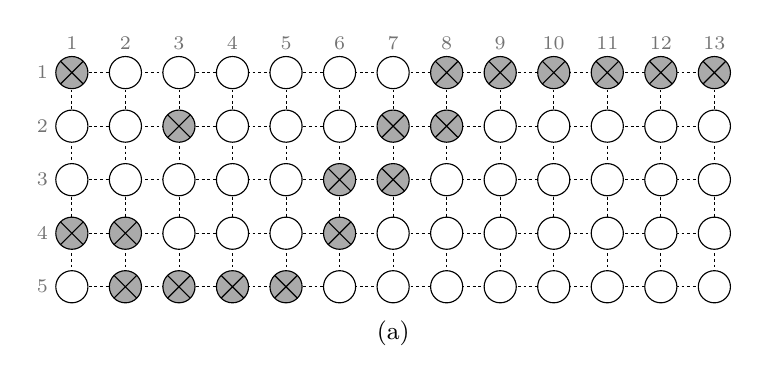
\begin{tikzpicture}[x=0.68cm,y=0.68cm,baseline=(current bounding box.north)]
  \begin{scope}[xshift=0.000cm]
    \draw[black,line width=0.27pt,dash pattern=on 1.02pt off 1.02pt] (1,-1) -- (13,-1) (1,-2) -- (13,-2) (1,-3) -- (13,-3) (1,-4) -- (13,-4) (1,-5) -- (13,-5) (1,-1) -- (1,-5) (2,-1) -- (2,-5) (3,-1) -- (3,-5) (4,-1) -- (4,-5) (5,-1) -- (5,-5) (6,-1) -- (6,-5) (7,-1) -- (7,-5) (8,-1) -- (8,-5) (9,-1) -- (9,-5) (10,-1) -- (10,-5) (11,-1) -- (11,-5) (12,-1) -- (12,-5) (13,-1) -- (13,-5);
    \filldraw[fill=kgray,draw=black,line width=0.41pt] (1,-1) circle (0.3);
    \draw[black,line width=0.41pt] (0.788,-0.788) -- (1.212,-1.212) (0.788,-1.212) -- (1.212,-0.788);
    \filldraw[fill=white,draw=black,line width=0.41pt] (2,-1) circle (0.3);
    \filldraw[fill=white,draw=black,line width=0.41pt] (3,-1) circle (0.3);
    \filldraw[fill=white,draw=black,line width=0.41pt] (4,-1) circle (0.3);
    \filldraw[fill=white,draw=black,line width=0.41pt] (5,-1) circle (0.3);
    \filldraw[fill=white,draw=black,line width=0.41pt] (6,-1) circle (0.3);
    \filldraw[fill=white,draw=black,line width=0.41pt] (7,-1) circle (0.3);
    \filldraw[fill=kgray,draw=black,line width=0.41pt] (8,-1) circle (0.3);
    \draw[black,line width=0.41pt] (7.788,-0.788) -- (8.212,-1.212) (7.788,-1.212) -- (8.212,-0.788);
    \filldraw[fill=kgray,draw=black,line width=0.41pt] (9,-1) circle (0.3);
    \draw[black,line width=0.41pt] (8.788,-0.788) -- (9.212,-1.212) (8.788,-1.212) -- (9.212,-0.788);
    \filldraw[fill=kgray,draw=black,line width=0.41pt] (10,-1) circle (0.3);
    \draw[black,line width=0.41pt] (9.788,-0.788) -- (10.212,-1.212) (9.788,-1.212) -- (10.212,-0.788);
    \filldraw[fill=kgray,draw=black,line width=0.41pt] (11,-1) circle (0.3);
    \draw[black,line width=0.41pt] (10.788,-0.788) -- (11.212,-1.212) (10.788,-1.212) -- (11.212,-0.788);
    \filldraw[fill=kgray,draw=black,line width=0.41pt] (12,-1) circle (0.3);
    \draw[black,line width=0.41pt] (11.788,-0.788) -- (12.212,-1.212) (11.788,-1.212) -- (12.212,-0.788);
    \filldraw[fill=kgray,draw=black,line width=0.41pt] (13,-1) circle (0.3);
    \draw[black,line width=0.41pt] (12.788,-0.788) -- (13.212,-1.212) (12.788,-1.212) -- (13.212,-0.788);
    \filldraw[fill=white,draw=black,line width=0.41pt] (1,-2) circle (0.3);
    \filldraw[fill=white,draw=black,line width=0.41pt] (2,-2) circle (0.3);
    \filldraw[fill=kgray,draw=black,line width=0.41pt] (3,-2) circle (0.3);
    \draw[black,line width=0.41pt] (2.788,-1.788) -- (3.212,-2.212) (2.788,-2.212) -- (3.212,-1.788);
    \filldraw[fill=white,draw=black,line width=0.41pt] (4,-2) circle (0.3);
    \filldraw[fill=white,draw=black,line width=0.41pt] (5,-2) circle (0.3);
    \filldraw[fill=white,draw=black,line width=0.41pt] (6,-2) circle (0.3);
    \filldraw[fill=kgray,draw=black,line width=0.41pt] (7,-2) circle (0.3);
    \draw[black,line width=0.41pt] (6.788,-1.788) -- (7.212,-2.212) (6.788,-2.212) -- (7.212,-1.788);
    \filldraw[fill=kgray,draw=black,line width=0.41pt] (8,-2) circle (0.3);
    \draw[black,line width=0.41pt] (7.788,-1.788) -- (8.212,-2.212) (7.788,-2.212) -- (8.212,-1.788);
    \filldraw[fill=white,draw=black,line width=0.41pt] (9,-2) circle (0.3);
    \filldraw[fill=white,draw=black,line width=0.41pt] (10,-2) circle (0.3);
    \filldraw[fill=white,draw=black,line width=0.41pt] (11,-2) circle (0.3);
    \filldraw[fill=white,draw=black,line width=0.41pt] (12,-2) circle (0.3);
    \filldraw[fill=white,draw=black,line width=0.41pt] (13,-2) circle (0.3);
    \filldraw[fill=white,draw=black,line width=0.41pt] (1,-3) circle (0.3);
    \filldraw[fill=white,draw=black,line width=0.41pt] (2,-3) circle (0.3);
    \filldraw[fill=white,draw=black,line width=0.41pt] (3,-3) circle (0.3);
    \filldraw[fill=white,draw=black,line width=0.41pt] (4,-3) circle (0.3);
    \filldraw[fill=white,draw=black,line width=0.41pt] (5,-3) circle (0.3);
    \filldraw[fill=kgray,draw=black,line width=0.41pt] (6,-3) circle (0.3);
    \draw[black,line width=0.41pt] (5.788,-2.788) -- (6.212,-3.212) (5.788,-3.212) -- (6.212,-2.788);
    \filldraw[fill=kgray,draw=black,line width=0.41pt] (7,-3) circle (0.3);
    \draw[black,line width=0.41pt] (6.788,-2.788) -- (7.212,-3.212) (6.788,-3.212) -- (7.212,-2.788);
    \filldraw[fill=white,draw=black,line width=0.41pt] (8,-3) circle (0.3);
    \filldraw[fill=white,draw=black,line width=0.41pt] (9,-3) circle (0.3);
    \filldraw[fill=white,draw=black,line width=0.41pt] (10,-3) circle (0.3);
    \filldraw[fill=white,draw=black,line width=0.41pt] (11,-3) circle (0.3);
    \filldraw[fill=white,draw=black,line width=0.41pt] (12,-3) circle (0.3);
    \filldraw[fill=white,draw=black,line width=0.41pt] (13,-3) circle (0.3);
    \filldraw[fill=kgray,draw=black,line width=0.41pt] (1,-4) circle (0.3);
    \draw[black,line width=0.41pt] (0.788,-3.788) -- (1.212,-4.212) (0.788,-4.212) -- (1.212,-3.788);
    \filldraw[fill=kgray,draw=black,line width=0.41pt] (2,-4) circle (0.3);
    \draw[black,line width=0.41pt] (1.788,-3.788) -- (2.212,-4.212) (1.788,-4.212) -- (2.212,-3.788);
    \filldraw[fill=white,draw=black,line width=0.41pt] (3,-4) circle (0.3);
    \filldraw[fill=white,draw=black,line width=0.41pt] (4,-4) circle (0.3);
    \filldraw[fill=white,draw=black,line width=0.41pt] (5,-4) circle (0.3);
    \filldraw[fill=kgray,draw=black,line width=0.41pt] (6,-4) circle (0.3);
    \draw[black,line width=0.41pt] (5.788,-3.788) -- (6.212,-4.212) (5.788,-4.212) -- (6.212,-3.788);
    \filldraw[fill=white,draw=black,line width=0.41pt] (7,-4) circle (0.3);
    \filldraw[fill=white,draw=black,line width=0.41pt] (8,-4) circle (0.3);
    \filldraw[fill=white,draw=black,line width=0.41pt] (9,-4) circle (0.3);
    \filldraw[fill=white,draw=black,line width=0.41pt] (10,-4) circle (0.3);
    \filldraw[fill=white,draw=black,line width=0.41pt] (11,-4) circle (0.3);
    \filldraw[fill=white,draw=black,line width=0.41pt] (12,-4) circle (0.3);
    \filldraw[fill=white,draw=black,line width=0.41pt] (13,-4) circle (0.3);
    \filldraw[fill=white,draw=black,line width=0.41pt] (1,-5) circle (0.3);
    \filldraw[fill=kgray,draw=black,line width=0.41pt] (2,-5) circle (0.3);
    \draw[black,line width=0.41pt] (1.788,-4.788) -- (2.212,-5.212) (1.788,-5.212) -- (2.212,-4.788);
    \filldraw[fill=kgray,draw=black,line width=0.41pt] (3,-5) circle (0.3);
    \draw[black,line width=0.41pt] (2.788,-4.788) -- (3.212,-5.212) (2.788,-5.212) -- (3.212,-4.788);
    \filldraw[fill=kgray,draw=black,line width=0.41pt] (4,-5) circle (0.3);
    \draw[black,line width=0.41pt] (3.788,-4.788) -- (4.212,-5.212) (3.788,-5.212) -- (4.212,-4.788);
    \filldraw[fill=kgray,draw=black,line width=0.41pt] (5,-5) circle (0.3);
    \draw[black,line width=0.41pt] (4.788,-4.788) -- (5.212,-5.212) (4.788,-5.212) -- (5.212,-4.788);
    \filldraw[fill=white,draw=black,line width=0.41pt] (6,-5) circle (0.3);
    \filldraw[fill=white,draw=black,line width=0.41pt] (7,-5) circle (0.3);
    \filldraw[fill=white,draw=black,line width=0.41pt] (8,-5) circle (0.3);
    \filldraw[fill=white,draw=black,line width=0.41pt] (9,-5) circle (0.3);
    \filldraw[fill=white,draw=black,line width=0.41pt] (10,-5) circle (0.3);
    \filldraw[fill=white,draw=black,line width=0.41pt] (11,-5) circle (0.3);
    \filldraw[fill=white,draw=black,line width=0.41pt] (12,-5) circle (0.3);
    \filldraw[fill=white,draw=black,line width=0.41pt] (13,-5) circle (0.3);
    \node[lab] at (1,-0.45) {1};
    \node[lab] at (2,-0.45) {2};
    \node[lab] at (3,-0.45) {3};
    \node[lab] at (4,-0.45) {4};
    \node[lab] at (5,-0.45) {5};
    \node[lab] at (6,-0.45) {6};
    \node[lab] at (7,-0.45) {7};
    \node[lab] at (8,-0.45) {8};
    \node[lab] at (9,-0.45) {9};
    \node[lab] at (10,-0.45) {10};
    \node[lab] at (11,-0.45) {11};
    \node[lab] at (12,-0.45) {12};
    \node[lab] at (13,-0.45) {13};
    \node[lab] at (0.45,-1) {1};
    \node[lab] at (0.45,-2) {2};
    \node[lab] at (0.45,-3) {3};
    \node[lab] at (0.45,-4) {4};
    \node[lab] at (0.45,-5) {5};
    \node[capt,anchor=north] at (7.00,-5.45) {(a)};
  \end{scope}
\end{tikzpicture}
\par\medskip
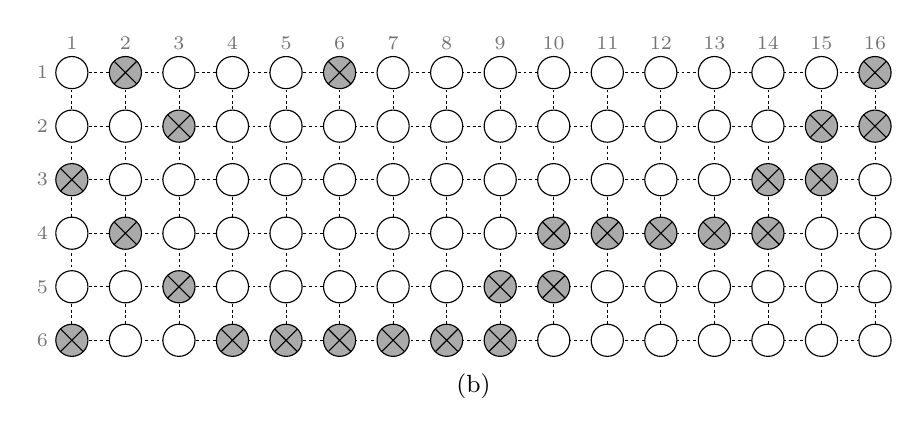
\begin{tikzpicture}[x=0.68cm,y=0.68cm,baseline=(current bounding box.north)]
  \begin{scope}[xshift=0.000cm]
    \draw[black,line width=0.27pt,dash pattern=on 1.02pt off 1.02pt] (1,-1) -- (16,-1) (1,-2) -- (16,-2) (1,-3) -- (16,-3) (1,-4) -- (16,-4) (1,-5) -- (16,-5) (1,-6) -- (16,-6) (1,-1) -- (1,-6) (2,-1) -- (2,-6) (3,-1) -- (3,-6) (4,-1) -- (4,-6) (5,-1) -- (5,-6) (6,-1) -- (6,-6) (7,-1) -- (7,-6) (8,-1) -- (8,-6) (9,-1) -- (9,-6) (10,-1) -- (10,-6) (11,-1) -- (11,-6) (12,-1) -- (12,-6) (13,-1) -- (13,-6) (14,-1) -- (14,-6) (15,-1) -- (15,-6) (16,-1) -- (16,-6);
    \filldraw[fill=white,draw=black,line width=0.41pt] (1,-1) circle (0.3);
    \filldraw[fill=kgray,draw=black,line width=0.41pt] (2,-1) circle (0.3);
    \draw[black,line width=0.41pt] (1.788,-0.788) -- (2.212,-1.212) (1.788,-1.212) -- (2.212,-0.788);
    \filldraw[fill=white,draw=black,line width=0.41pt] (3,-1) circle (0.3);
    \filldraw[fill=white,draw=black,line width=0.41pt] (4,-1) circle (0.3);
    \filldraw[fill=white,draw=black,line width=0.41pt] (5,-1) circle (0.3);
    \filldraw[fill=kgray,draw=black,line width=0.41pt] (6,-1) circle (0.3);
    \draw[black,line width=0.41pt] (5.788,-0.788) -- (6.212,-1.212) (5.788,-1.212) -- (6.212,-0.788);
    \filldraw[fill=white,draw=black,line width=0.41pt] (7,-1) circle (0.3);
    \filldraw[fill=white,draw=black,line width=0.41pt] (8,-1) circle (0.3);
    \filldraw[fill=white,draw=black,line width=0.41pt] (9,-1) circle (0.3);
    \filldraw[fill=white,draw=black,line width=0.41pt] (10,-1) circle (0.3);
    \filldraw[fill=white,draw=black,line width=0.41pt] (11,-1) circle (0.3);
    \filldraw[fill=white,draw=black,line width=0.41pt] (12,-1) circle (0.3);
    \filldraw[fill=white,draw=black,line width=0.41pt] (13,-1) circle (0.3);
    \filldraw[fill=white,draw=black,line width=0.41pt] (14,-1) circle (0.3);
    \filldraw[fill=white,draw=black,line width=0.41pt] (15,-1) circle (0.3);
    \filldraw[fill=kgray,draw=black,line width=0.41pt] (16,-1) circle (0.3);
    \draw[black,line width=0.41pt] (15.788,-0.788) -- (16.212,-1.212) (15.788,-1.212) -- (16.212,-0.788);
    \filldraw[fill=white,draw=black,line width=0.41pt] (1,-2) circle (0.3);
    \filldraw[fill=white,draw=black,line width=0.41pt] (2,-2) circle (0.3);
    \filldraw[fill=kgray,draw=black,line width=0.41pt] (3,-2) circle (0.3);
    \draw[black,line width=0.41pt] (2.788,-1.788) -- (3.212,-2.212) (2.788,-2.212) -- (3.212,-1.788);
    \filldraw[fill=white,draw=black,line width=0.41pt] (4,-2) circle (0.3);
    \filldraw[fill=white,draw=black,line width=0.41pt] (5,-2) circle (0.3);
    \filldraw[fill=white,draw=black,line width=0.41pt] (6,-2) circle (0.3);
    \filldraw[fill=white,draw=black,line width=0.41pt] (7,-2) circle (0.3);
    \filldraw[fill=white,draw=black,line width=0.41pt] (8,-2) circle (0.3);
    \filldraw[fill=white,draw=black,line width=0.41pt] (9,-2) circle (0.3);
    \filldraw[fill=white,draw=black,line width=0.41pt] (10,-2) circle (0.3);
    \filldraw[fill=white,draw=black,line width=0.41pt] (11,-2) circle (0.3);
    \filldraw[fill=white,draw=black,line width=0.41pt] (12,-2) circle (0.3);
    \filldraw[fill=white,draw=black,line width=0.41pt] (13,-2) circle (0.3);
    \filldraw[fill=white,draw=black,line width=0.41pt] (14,-2) circle (0.3);
    \filldraw[fill=kgray,draw=black,line width=0.41pt] (15,-2) circle (0.3);
    \draw[black,line width=0.41pt] (14.788,-1.788) -- (15.212,-2.212) (14.788,-2.212) -- (15.212,-1.788);
    \filldraw[fill=kgray,draw=black,line width=0.41pt] (16,-2) circle (0.3);
    \draw[black,line width=0.41pt] (15.788,-1.788) -- (16.212,-2.212) (15.788,-2.212) -- (16.212,-1.788);
    \filldraw[fill=kgray,draw=black,line width=0.41pt] (1,-3) circle (0.3);
    \draw[black,line width=0.41pt] (0.788,-2.788) -- (1.212,-3.212) (0.788,-3.212) -- (1.212,-2.788);
    \filldraw[fill=white,draw=black,line width=0.41pt] (2,-3) circle (0.3);
    \filldraw[fill=white,draw=black,line width=0.41pt] (3,-3) circle (0.3);
    \filldraw[fill=white,draw=black,line width=0.41pt] (4,-3) circle (0.3);
    \filldraw[fill=white,draw=black,line width=0.41pt] (5,-3) circle (0.3);
    \filldraw[fill=white,draw=black,line width=0.41pt] (6,-3) circle (0.3);
    \filldraw[fill=white,draw=black,line width=0.41pt] (7,-3) circle (0.3);
    \filldraw[fill=white,draw=black,line width=0.41pt] (8,-3) circle (0.3);
    \filldraw[fill=white,draw=black,line width=0.41pt] (9,-3) circle (0.3);
    \filldraw[fill=white,draw=black,line width=0.41pt] (10,-3) circle (0.3);
    \filldraw[fill=white,draw=black,line width=0.41pt] (11,-3) circle (0.3);
    \filldraw[fill=white,draw=black,line width=0.41pt] (12,-3) circle (0.3);
    \filldraw[fill=white,draw=black,line width=0.41pt] (13,-3) circle (0.3);
    \filldraw[fill=kgray,draw=black,line width=0.41pt] (14,-3) circle (0.3);
    \draw[black,line width=0.41pt] (13.788,-2.788) -- (14.212,-3.212) (13.788,-3.212) -- (14.212,-2.788);
    \filldraw[fill=kgray,draw=black,line width=0.41pt] (15,-3) circle (0.3);
    \draw[black,line width=0.41pt] (14.788,-2.788) -- (15.212,-3.212) (14.788,-3.212) -- (15.212,-2.788);
    \filldraw[fill=white,draw=black,line width=0.41pt] (16,-3) circle (0.3);
    \filldraw[fill=white,draw=black,line width=0.41pt] (1,-4) circle (0.3);
    \filldraw[fill=kgray,draw=black,line width=0.41pt] (2,-4) circle (0.3);
    \draw[black,line width=0.41pt] (1.788,-3.788) -- (2.212,-4.212) (1.788,-4.212) -- (2.212,-3.788);
    \filldraw[fill=white,draw=black,line width=0.41pt] (3,-4) circle (0.3);
    \filldraw[fill=white,draw=black,line width=0.41pt] (4,-4) circle (0.3);
    \filldraw[fill=white,draw=black,line width=0.41pt] (5,-4) circle (0.3);
    \filldraw[fill=white,draw=black,line width=0.41pt] (6,-4) circle (0.3);
    \filldraw[fill=white,draw=black,line width=0.41pt] (7,-4) circle (0.3);
    \filldraw[fill=white,draw=black,line width=0.41pt] (8,-4) circle (0.3);
    \filldraw[fill=white,draw=black,line width=0.41pt] (9,-4) circle (0.3);
    \filldraw[fill=kgray,draw=black,line width=0.41pt] (10,-4) circle (0.3);
    \draw[black,line width=0.41pt] (9.788,-3.788) -- (10.212,-4.212) (9.788,-4.212) -- (10.212,-3.788);
    \filldraw[fill=kgray,draw=black,line width=0.41pt] (11,-4) circle (0.3);
    \draw[black,line width=0.41pt] (10.788,-3.788) -- (11.212,-4.212) (10.788,-4.212) -- (11.212,-3.788);
    \filldraw[fill=kgray,draw=black,line width=0.41pt] (12,-4) circle (0.3);
    \draw[black,line width=0.41pt] (11.788,-3.788) -- (12.212,-4.212) (11.788,-4.212) -- (12.212,-3.788);
    \filldraw[fill=kgray,draw=black,line width=0.41pt] (13,-4) circle (0.3);
    \draw[black,line width=0.41pt] (12.788,-3.788) -- (13.212,-4.212) (12.788,-4.212) -- (13.212,-3.788);
    \filldraw[fill=kgray,draw=black,line width=0.41pt] (14,-4) circle (0.3);
    \draw[black,line width=0.41pt] (13.788,-3.788) -- (14.212,-4.212) (13.788,-4.212) -- (14.212,-3.788);
    \filldraw[fill=white,draw=black,line width=0.41pt] (15,-4) circle (0.3);
    \filldraw[fill=white,draw=black,line width=0.41pt] (16,-4) circle (0.3);
    \filldraw[fill=white,draw=black,line width=0.41pt] (1,-5) circle (0.3);
    \filldraw[fill=white,draw=black,line width=0.41pt] (2,-5) circle (0.3);
    \filldraw[fill=kgray,draw=black,line width=0.41pt] (3,-5) circle (0.3);
    \draw[black,line width=0.41pt] (2.788,-4.788) -- (3.212,-5.212) (2.788,-5.212) -- (3.212,-4.788);
    \filldraw[fill=white,draw=black,line width=0.41pt] (4,-5) circle (0.3);
    \filldraw[fill=white,draw=black,line width=0.41pt] (5,-5) circle (0.3);
    \filldraw[fill=white,draw=black,line width=0.41pt] (6,-5) circle (0.3);
    \filldraw[fill=white,draw=black,line width=0.41pt] (7,-5) circle (0.3);
    \filldraw[fill=white,draw=black,line width=0.41pt] (8,-5) circle (0.3);
    \filldraw[fill=kgray,draw=black,line width=0.41pt] (9,-5) circle (0.3);
    \draw[black,line width=0.41pt] (8.788,-4.788) -- (9.212,-5.212) (8.788,-5.212) -- (9.212,-4.788);
    \filldraw[fill=kgray,draw=black,line width=0.41pt] (10,-5) circle (0.3);
    \draw[black,line width=0.41pt] (9.788,-4.788) -- (10.212,-5.212) (9.788,-5.212) -- (10.212,-4.788);
    \filldraw[fill=white,draw=black,line width=0.41pt] (11,-5) circle (0.3);
    \filldraw[fill=white,draw=black,line width=0.41pt] (12,-5) circle (0.3);
    \filldraw[fill=white,draw=black,line width=0.41pt] (13,-5) circle (0.3);
    \filldraw[fill=white,draw=black,line width=0.41pt] (14,-5) circle (0.3);
    \filldraw[fill=white,draw=black,line width=0.41pt] (15,-5) circle (0.3);
    \filldraw[fill=white,draw=black,line width=0.41pt] (16,-5) circle (0.3);
    \filldraw[fill=kgray,draw=black,line width=0.41pt] (1,-6) circle (0.3);
    \draw[black,line width=0.41pt] (0.788,-5.788) -- (1.212,-6.212) (0.788,-6.212) -- (1.212,-5.788);
    \filldraw[fill=white,draw=black,line width=0.41pt] (2,-6) circle (0.3);
    \filldraw[fill=white,draw=black,line width=0.41pt] (3,-6) circle (0.3);
    \filldraw[fill=kgray,draw=black,line width=0.41pt] (4,-6) circle (0.3);
    \draw[black,line width=0.41pt] (3.788,-5.788) -- (4.212,-6.212) (3.788,-6.212) -- (4.212,-5.788);
    \filldraw[fill=kgray,draw=black,line width=0.41pt] (5,-6) circle (0.3);
    \draw[black,line width=0.41pt] (4.788,-5.788) -- (5.212,-6.212) (4.788,-6.212) -- (5.212,-5.788);
    \filldraw[fill=kgray,draw=black,line width=0.41pt] (6,-6) circle (0.3);
    \draw[black,line width=0.41pt] (5.788,-5.788) -- (6.212,-6.212) (5.788,-6.212) -- (6.212,-5.788);
    \filldraw[fill=kgray,draw=black,line width=0.41pt] (7,-6) circle (0.3);
    \draw[black,line width=0.41pt] (6.788,-5.788) -- (7.212,-6.212) (6.788,-6.212) -- (7.212,-5.788);
    \filldraw[fill=kgray,draw=black,line width=0.41pt] (8,-6) circle (0.3);
    \draw[black,line width=0.41pt] (7.788,-5.788) -- (8.212,-6.212) (7.788,-6.212) -- (8.212,-5.788);
    \filldraw[fill=kgray,draw=black,line width=0.41pt] (9,-6) circle (0.3);
    \draw[black,line width=0.41pt] (8.788,-5.788) -- (9.212,-6.212) (8.788,-6.212) -- (9.212,-5.788);
    \filldraw[fill=white,draw=black,line width=0.41pt] (10,-6) circle (0.3);
    \filldraw[fill=white,draw=black,line width=0.41pt] (11,-6) circle (0.3);
    \filldraw[fill=white,draw=black,line width=0.41pt] (12,-6) circle (0.3);
    \filldraw[fill=white,draw=black,line width=0.41pt] (13,-6) circle (0.3);
    \filldraw[fill=white,draw=black,line width=0.41pt] (14,-6) circle (0.3);
    \filldraw[fill=white,draw=black,line width=0.41pt] (15,-6) circle (0.3);
    \filldraw[fill=white,draw=black,line width=0.41pt] (16,-6) circle (0.3);
    \node[lab] at (1,-0.45) {1};
    \node[lab] at (2,-0.45) {2};
    \node[lab] at (3,-0.45) {3};
    \node[lab] at (4,-0.45) {4};
    \node[lab] at (5,-0.45) {5};
    \node[lab] at (6,-0.45) {6};
    \node[lab] at (7,-0.45) {7};
    \node[lab] at (8,-0.45) {8};
    \node[lab] at (9,-0.45) {9};
    \node[lab] at (10,-0.45) {10};
    \node[lab] at (11,-0.45) {11};
    \node[lab] at (12,-0.45) {12};
    \node[lab] at (13,-0.45) {13};
    \node[lab] at (14,-0.45) {14};
    \node[lab] at (15,-0.45) {15};
    \node[lab] at (16,-0.45) {16};
    \node[lab] at (0.45,-1) {1};
    \node[lab] at (0.45,-2) {2};
    \node[lab] at (0.45,-3) {3};
    \node[lab] at (0.45,-4) {4};
    \node[lab] at (0.45,-5) {5};
    \node[lab] at (0.45,-6) {6};
    \node[capt,anchor=north] at (8.50,-6.45) {(b)};
  \end{scope}
\end{tikzpicture}
\caption{(a) The $5\times13$ test board of $S_8$. (b) The $6\times16$ blackout $S_{16}$.}
\label{fig:boards}
\end{figure}

\begin{theorem}[five rows, (a) and (c) computer-assisted, (b) checked in Lean]\label{thm:fiverow}
\leavevmode
\begin{enumerate}[(a)]
\item We have $f(5,m)=m+5$ for $m=5$, $6$, and $7$.
\item We have $f(5,m)=m+6$ for every $m\ge8$, attained by $S_8$ followed by $m-8$ columns black in
row $1$ only.
\item The $5\times8$ grid has exactly four maximum blackouts, the images of $S_8$ under row
reflection and column reversal.
\end{enumerate}
\end{theorem}

\begin{proof}
(b) The upper bound is Theorem~\ref{thm:rowbound}.
For the construction, $W_5=5$, so the collar theorem with right padding
in row $1$ reduces the whole family from $S_8$ to Figure~\ref{fig:boards}(a).
Three enumerators and Lean verify that the $954$ rectangles of this
test board have different presentations.
(a) At $m=5$, use Corollary~\ref{cor:small-m} and the construction $S_0$
in Theorem~\ref{thm:fivefive}. At $m=6,7$, the constructions are
$15,\allowbreak 12,\allowbreak 23,\allowbreak 3,\allowbreak 34,\allowbreak 45$ and
$1,\allowbreak 12,\allowbreak 23,\allowbreak 3,\allowbreak 34,\allowbreak 45,\allowbreak 15$,
recorded in \nolinkurl{jis/data/small_cells_sat_5x6.json} and
\nolinkurl{jis/data/small_cells_sat_5x7_b12.json}. They give the lower
bounds. Checked SAT certificates rule out $m+6$ points
(Section~\ref{sec:verify}).
(c) Two SAT enumerations find the four images. A separate column search
checks all $10\,(8)_6\,5^2=5{,}040{,}000$ equality candidates from
Theorem~\ref{thm:equality} and finds the same four.
\end{proof}

Theorem~\ref{thm:A} gives $f(h,m)\le h+m$ whenever a side is at most
four, and on $5\times5$, $5\times6$, $5\times7$, and $6\times6$.
Up to transposition, these exhaust the grids of area below $40$.
Thus $5\times8$ is the first failure of the guess $f(h,m)=h+m$.

\begin{remark}[five-row counts, computer-assisted]\label{rem:fivecounts}
For $m=13,\dots,23$ the counts $a_5(m)$ are
\begin{gather*}
193{,}406,\quad 1{,}346{,}758,\quad 8{,}650{,}416,\quad 52{,}128{,}242,\\
299{,}349{,}210,\quad 1{,}653{,}637{,}492,\quad 8{,}828{,}301{,}226,\quad 45{,}743{,}165{,}894,\\
230{,}934{,}909{,}328,\quad 1{,}139{,}486{,}126{,}866,\quad 5{,}510{,}071{,}794{,}736.
\end{gather*}
Each count agrees in two independent transfer calculations using the
equality structure of Theorem~\ref{thm:equality}.
\end{remark}

\subsection{Six rows and small grids}

Let $S_{16}$ be the blackout of the $6\times16$ grid in Figure~\ref{fig:boards}(b). Its doubles,
in the columns $1,2,3,6,9,10,14,15,16$, carry the edges of $K_{3,3}$ between $\{1,3,5\}$ and
$\{2,4,6\}$.

\begin{theorem}[six rows, (a) computer-assisted, (b) checked in Lean]\label{thm:sixrow}
\leavevmode
\begin{enumerate}[(a)]
\item For $8\le m\le14$ we have $f(6,m)\le m+8$.
\item For every $m\ge15$ we have $f(6,m)=m+9$.
\end{enumerate}
\end{theorem}

\begin{proof}
(a) Corollary~\ref{cor:small-m} handles $m=8$.
For $9\le m\le14$, an optimum with $m+9$ points would have double
columns carrying $K_{3,3}$, by Theorem~\ref{thm:equality}.
There are ten possible row partitions. The structured encoding has
checked LRAT certificates excluding every one (Lemma~\ref{lem:enc}).
(b) Again the row bound gives the upper bound. For $m=15$, take
$56,\allowbreak 45,\allowbreak 34,\allowbreak 23,\allowbreak 1,\allowbreak 1,\allowbreak 14,\allowbreak 1,\allowbreak 1,\allowbreak 12,\allowbreak 36,\allowbreak 1,\allowbreak 25,\allowbreak 6,\allowbreak 16$
from \nolinkurl{jis/data/six_row_sat_w15_A.json}, which is valid with
$24$ points. For $m\ge16$, apply the collar theorem to $S_{16}$ in
Figure~\ref{fig:boards}(b). Since $W_6=7$, it suffices to add
$(17,1),\dots,(23,1)$. Three enumerators and Lean verify distinct
presentations for all $4{,}627$ rectangles of that test board.
\end{proof}

\begin{theorem}[small grids, computer-assisted]\label{thm:refute}
We have $f(6,6)=12$, $f(6,7)=13$, $f(7,7)=14$, and $f(6,8)=15$. The blackout
$15,\allowbreak 1,\allowbreak 123,\allowbreak 34,\allowbreak 4,\allowbreak 4,\allowbreak 456,\allowbreak 26$ of the $6\times8$ grid attains the last value.
\end{theorem}

\begin{proof}
The other constructions are $14,\allowbreak 1,\allowbreak 12,\allowbreak 2,\allowbreak 23,\allowbreak 3456$
on the $6\times6$ grid,
$16,\allowbreak 1,\allowbreak 1,\allowbreak 12,\allowbreak 2,\allowbreak 23,\allowbreak 3456$
on $6\times7$, and
$17,\allowbreak 1,\allowbreak 12,\allowbreak 2,\allowbreak 23,\allowbreak 3456,\allowbreak 67$
on $7\times7$. Their records are
\nolinkurl{jis/data/small_cells_sat_6x6.json},
\nolinkurl{jis/data/small_cells_sat_6x7.json}, and
\nolinkurl{jis/data/small_cells_sat_7x7.json}.
All are valid. For each grid, a checked SAT certificate excludes
one additional point.
\end{proof}

\begin{theorem}[the $5\times5$ grid]\label{thm:fivefive}
\leavevmode
\begin{enumerate}[(a)]
\item We have $f(5,5)=10$.
\item (Computer-assisted.) The $a_5(5)=8$ maximum blackouts are the images of $S_0$
below under the square's symmetries.
\end{enumerate}
\end{theorem}

\begin{proof}
(a) Corollary~\ref{cor:small-m} gives the upper bound. To attain it,
take $S_0$ to be $45,\allowbreak 34,\allowbreak 123,\allowbreak 1,\allowbreak 15$.
Its row-column graph is an $8$-cycle with two pendant edges, hence it is
axis-valid. Lemma~\ref{lem:leftmost} lists $30$ tilted rectangles, namely
nine unit diamonds, sixteen others from Lemma~\ref{lem:tilted-narrow},
and five spanning the grid. The fifteen weak rectangles show the pairs
below. After an oblique pair, the point following the bar is a white
corner of the axis-aligned rectangle through it.
\begin{center}\footnotesize
\begin{tabular}{@{}llll@{}}
$(1,2),(2,1)\mid(1,1)$ & $(1,3),(2,2)\mid(1,2)$ & $(3,4),(4,3)\mid(4,4)$ & $(2,5),(3,4)\mid(3,5)$ \\
$(2,2),(4,2)$ & $(1,2),(4,3)\mid(1,3)$ & $(4,4),(5,2)\mid(4,2)$ & $(3,5),(4,4)\mid(3,4)$ \\
$(4,3),(5,2)\mid(4,2)$ & $(3,4),(5,2)\mid(5,4)$ & $(2,5),(5,2)\mid(2,2)$ & $(4,5),(5,3)\mid(4,3)$ \\
$(1,3),(4,2)\mid(1,2)$ & $(2,5),(4,3)\mid(4,5)$ & & $(4,5),(5,4)\mid(4,4)$ \\
\end{tabular}
\end{center}
These pairs are all different. The other tilted rectangles show at least
three points, so Lemma~\ref{lem:threecorners} distinguishes them.
The listed white corners rule out axis-aligned rivals for every oblique
pair. The remaining pair $(2,2),(4,2)$ has no rival because
$B_2\cap B_4=\emptyset$. This proves validity.
(b) Three programs check all $44{,}640$ sets of $10$ points whose graph
has no four- or six-cycle. Only the images of $S_0$ are valid.
\end{proof}
\section{Every fixed height}\label{sec:height}

Fix the height $h$ and read the grid from left to right. Its blackout is
the \emph{column word} $w=B_1\cdots B_m$, whose letter $B_i$ records the
black rows in column $i$. Write $|w|=m$ and $S(w)$ for its blackout, and
let $\mathcal L_h$ be the valid words, including the empty word. We first
show that validity needs only finite memory. A bounded counter will then
pick out the words with the most black points.

\begin{theorem}[regularity and rational series]\label{thm:regular}
For every $h\ge1$ the language $\mathcal L_h$ is regular, and $G_h(z,u)=\sum_{w\in\mathcal L_h}z^{|w|}u^{|S(w)|}$ is rational in $z$ and $u$.
\end{theorem}

\begin{proof}
The \emph{trace} of a rectangle records, in each column, the rows of its
corners. It determines the corner set. By Lemma~\ref{lem:diff}, two distinct
traces $Y,Y'$ give the same presentation exactly when
$Y_i\triangle Y'_i\subseteq B_i$ in every column.

The possible traces form a regular language. For an axis-aligned rectangle,
choose $r<s$, read a column $\{r,s\}$, then another such column after any
number of empty columns. There can also be empty columns before and after.
For a tilted rectangle, Lemmas~\ref{lem:leftmost} and~\ref{lem:span} leave
only finitely many templates~\eqref{eq:tilt-param}, each of span at most
$W_h$, again with arbitrary empty columns on either side.

An automaton can therefore read $w$ while guessing two rectangle traces.
It checks the containment above and remembers whether the traces have
differed anywhere. Accepting when they differ recognizes the invalid words.
Regular languages are closed under complementation, so $\mathcal L_h$ is
regular too.

Choose a deterministic automaton for $\mathcal L_h$ and give a transition
reading $B$ the weight $u^{|B|}$. If $M(u)$ is its weighted transition
matrix, $\alpha$ its start vector and $\beta$ its accepting vector, then
\[
 G_h(z,u)=\alpha(I-zM(u))^{-1}\beta .
\]
Each word is counted once because the automaton is deterministic. Cramer's
rule makes the expression rational~\cite[Proposition~V.6]{flajolet2009}.
\end{proof}

\begin{theorem}[fixed height]\label{thm:periodic}
Let $h\ge2$. (a) There are integers $m_0\ge3$, $p\ge1$, and $k_0,\dots,k_{p-1}$ such that $f(h,m)=m+k_{m\bmod p}$ for every $m\ge m_0$. (b) The series $\sum_{m\ge0}a_h(m)z^m$ is rational, with the conventions of Section~\ref{sec:conv}, and the words of optimum blackouts form a regular language.
\end{theorem}

\begin{proof}
Put $E(w)=|S(w)|-|w|$, the number of black points beyond one per column.
Every consecutive block $v$ of a valid word is valid on its own grid.
Theorem~\ref{thm:rowbound} bounds $E(v)$ by $q_h$ when $|v|\ge3$.
For a shorter block, $|S(v)|\le h|v|$ gives the common bound
\[
 E(v)\le C_h:=\max(q_h,2h-2).
\]
If a valid word $w=uv$ has excess $k$, applying this to the prefix and
suffix gives
\[
 k-C_h\le E(u)=k-E(v)\le C_h.
\]
Thus, for a fixed $k$, only finitely many prefix excesses need to be
remembered. Add this counter to an automaton for $\mathcal L_h$, and
accept when the final excess is $k$. It recognizes the regular language
$\mathcal L_{h,k}$ of valid words with that excess.

The set of lengths of a regular language is eventually periodic. For
$m\ge3$, Lemma~\ref{lem:cross} and Theorem~\ref{thm:rowbound} put the
optimal excess between $h-1$ and $q_h$. There are only finitely many such
$k$, so choose one common period $p$ and threshold $m_0$ for their length
sets. The largest available excess then depends only on $m\bmod p$.
Calling it $k_r$ proves (a).

For each residue $r$, keep the words of $\mathcal L_{h,k_r}$ whose lengths
are at least $m_0$ and congruent to $r$ modulo $p$. This is still a regular
language. Their union, together with the finitely many shorter optimum
words, is exactly the language of optimum blackouts. Its counting series
is rational by the same transfer-matrix argument as above, proving (b).
\end{proof}
\section{Computations and verification}\label{sec:verify}

Every computed maximum and exact count has two separately written
checks. The bound $a_7(8)\ge18$, obtained by
one enumeration. The repository~\cite{repo} stores the code and
evidence. All paths here start from \nolinkurl{kagey-problems/problem001}.
For commands, SHA-256 hashes, and running times, see
\nolinkurl{jis/scripts/README.md}. Table~\ref{tab:evidence} connects
each computer-assisted claim to its checks.

We solve the hitting-set problem of Lemma~\ref{lem:diff} by ILP,
using CBC~\cite{cbc} through PuLP~\cite{pulp}, and check it by brute
force. SAT enumeration uses PySAT~\cite{pysat2018}.
The column searches grow the board from left to right. They use
$f(6,6)\le12$ to prune $6\times7$ and $6\times8$, and
$f(6,7)\le13$ to prune $6\times8$ and $7\times7$.
Every saved construction and counted model is tested for validity.

\begin{table}[!htb]
\centering\scriptsize\setlength{\tabcolsep}{3pt}
\begin{tabular}{@{}lrrl@{}}
\toprule
grid & $f$ & $a_h(m)$ & by \\
\midrule
$2\times2$ & $4$ & $1$ & HIB \\
$2\times3$ & $4$ & $12$ & HIB \\
$2\times4$ & $5$ & $32$ & HIB \\
$2\times5$ & $6$ & $80$ & IB \\
$2\times6$ & $7$ & $192$ & TI \\
$2\times7$ & $8$ & $448$ & TI \\
$3\times3$ & $5$ & $53$ & IB \\
$3\times4$ & $6$ & $224$ & IB \\
$3\times5$ & $7$ & $892$ & IB \\
$3\times6$ & $8$ & $3{,}420$ & IB \\
$3\times7$ & $9$ & $12{,}704$ & IB \\
\bottomrule
\end{tabular}\hspace{1.5em}
\begin{tabular}{@{}lrrl@{}}
\toprule
grid & $f$ & $a_h(m)$ & by \\
\midrule
$3\times8$ & $10$ & $45{,}864$ & IB \\
$3\times9$ & $11$ & $161{,}992$ & IB \\
$3\times10$ & $12$ & $562{,}912$ & ITD \\
$4\times4$ & $7$ & $316$ & IB \\
$4\times5$ & $8$ & $1{,}810$ & IB \\
$4\times6$ & $10$ & $26$ & IB \\
$4\times7$ & $11$ & $292$ & IB \\
$4\times8$ & $12$ & $2{,}118$ & IMD \\
$5\times5$ & $10$ & $8$ & IB \\
$5\times6$ & $11$ & $76$ & ISC \\
$5\times7$ & $12$ & $1{,}184$ & ISC \\
\bottomrule
\end{tabular}\hspace{1.5em}
\begin{tabular}{@{}lrrl@{}}
\toprule
grid & $f$ & $a_h(m)$ & by \\
\midrule
$5\times8$ & $14$ & $4$ & TSDC \\
$5\times9$ & $15$ & $44$ & TSC \\
$5\times10$ & $16$ & $350$ & TSC \\
$5\times11$ & $17$ & $3{,}004$ & TSC \\
$5\times12$ & $18$ & $24{,}706$ & TSCM \\
$6\times6$ & $12$ & $160$ & ISC \\
$6\times7$ & $13$ & $2{,}536$ & SC \\
$6\times8$ & $15$ & $8$ & SC \\
$6\times15$ & $24$ & -- & TS \\
$7\times7$ & $14$ & $7{,}300$ & SC \\
$7\times8$ & $16$ & $\ge18$ & S \\
\bottomrule
\end{tabular}
\caption{Computed values for $h\le m$. H: hand, T: theorem, I: ILP (value only on
$3\times10$, $4\times8$, $5\times6$, $5\times7$, and $6\times6$), B: brute force, D: equality
candidates, C: column search, S: two SAT encodings, with complete enumeration for exact
counts, M: transfer counter,
--: not established. On $7\times8$ only a lower bound for the count is given.}
\label{tab:values}
\end{table}

As a check on rectangle generation, the totals match
\seqnum{A085582} for squares and \seqnum{A289832} for rectangular grids.

Encoding A prevents the inclusion-minimal differences
$C(R_1)\triangle C(R_2)$, $R_1\ne R_2$, from being entirely black.
Encoding B forbids $C(R_1)\triangle C(R_2)$ only for distinct
rectangles with a common corner. Each rectangle $R$ also has an
indicator $y_R$, forced true if it is hidden, and at most one $y_R$
may be true.

For the structured six-row instances, fix a partition $A\mid B$
into triples. A column type is its black-row set, either a singleton
or one of the nine pairs meeting $A$ and $B$. Use each pair once.
Of encoding B's clauses, retain those involving a tilted rectangle
whose forbidden set can be all black. Cardinality is enforced by
Sinz's sequential counter~\cite{sinz2005}, expanded by our generator
for certified instances, or by a totalizer~\cite{bailleux2003}.
Both enforce exactly the specified size bound.

\begin{lemma}[faithful encodings]\label{lem:enc}
Let $S$ be a blackout of the $h\times m$ grid, and let
$\mathcal D=\{C(R_1)\triangle C(R_2)\mid R_1\ne R_2\}$, where $R_1$ and $R_2$ range over
rectangles of this grid.
\begin{enumerate}[(a)]
\item $S$ is valid if and only if it contains no inclusion-minimal member of $\mathcal D$.
\item $S$ is valid if and only if it hides at most one rectangle and contains no
$C(R_1)\triangle C(R_2)$ for distinct rectangles $R_1,R_2$ sharing a corner.
\item Suppose $h=6$, $m\ge3$, and $S$ is valid with $m+9$ points. For some partition of
the rows into two triples, selecting the black-row set $B_i$ as the type of column $i$
extends to a satisfying assignment of the structured instance.
\end{enumerate}
\end{lemma}

\begin{proof}
(a) Any member of the finite family $\mathcal D$ contains an
inclusion-minimal member. Thus a blackout contains a forbidden
difference exactly when it contains a minimal one. Apply
Corollary~\ref{cor:hitting}.

(b) Part (a) leaves only pairs with no shared corner to check.
For these, the difference is $C(R_1)\cup C(R_2)$, contained in $S$
exactly when both rectangles are hidden. Allowing at most one hidden
rectangle excludes precisely these remaining pairs.

(c) Theorem~\ref{thm:equality} gives a partition into two row triples.
Every $B_i$ is a singleton or a pair crossing it, and all nine pairs
occur once. Use these as the column types. Set $y_R$ to $1$ exactly
for hidden rectangles. By (b), these choices satisfy encoding B.
Dropping clauses preserves satisfaction in the structured instance.
\end{proof}

Reading the point variables of A or B therefore gives precisely the
valid blackouts of the chosen size. For six rows, part (c) and the
row bound imply $f(6,m)\le m+8$ once the ten structured instances of
width $m$ are all unsatisfiable.

CaDiCaL~\cite{biere2024} produces LRAT certificates for
$f(5,6)<12$, $f(5,7)<13$, $f(6,6)<13$, $f(6,7)<14$, $f(7,7)<15$,
$f(6,8)<16$, and $f(7,8)<17$ using encoding A on all blackouts.
It also certifies the $70$ structured six-row instances, for widths
$8$ to $14$ and ten partitions per width, in Theorem~\ref{thm:sixrow}(a).
The clauses agree between two independent generators.
We split $6\times8$ by its first column into $64$ cases, and
$7\times7$ and $7\times8$ into $128$ each. The second generator
checks that these splits exhaust the first-column choices.
Every one of the $394$ proofs passes both drat-trim's
\texttt{lrat-check}~\cite{cruzfilipe2017,wetzler2014} and the Lean
LRAT checker.

The constructions in \nolinkurl{jis/data/table_counts/sat_7x8_16.json}
give $f(7,8)\ge16$, completing $f(7,8)=16$.
The separate enumeration
\nolinkurl{jis/data/table_counts/sat2split_7x8_16.json} gives $18$
valid constructions with $16$ points. This proves only $a_7(8)\ge18$.

\begin{table}[!htb]
\centering\scriptsize\setlength{\tabcolsep}{3pt}
\begin{tabular}{@{}>{\raggedright\arraybackslash}p{0.3\textwidth}>{\raggedright\arraybackslash}p{0.3\textwidth}>{\raggedright\arraybackslash}p{0.36\textwidth}@{}}
\toprule
statement & method; independent check & evidence \\
\midrule
Cor.~\ref{cor:fourboundary}, Thm.~\ref{thm:fivefive}(b) & candidates; brute force & \nolinkurl{verify_narrow.py} \\
Thms.~\ref{thm:threegf}, \ref{thm:threeclosed}, Rem.~\ref{rem:threeorbits} & SymPy; transfer matrix & \nolinkurl{three_row_*.json} \\
Thm.~\ref{thm:fourgfexact}, Cor.~\ref{cor:fourgrowth}, Table~\ref{tab:fourvalues} & Prop.~\ref{prop:fourautomaton}; candidates & \nolinkurl{four_row_*.json} \\
Thms.~\ref{thm:fiverow}(a), \ref{thm:refute} & encoding A, LRAT; encoding B & \nolinkurl{unsat_certificates.json}, \nolinkurl{small_cells_*} \\
Thms.~\ref{thm:fiverow}(b), \ref{thm:sixrow}(b) & collar board; enumerators, Lean & \nolinkurl{five_row_*family*}, \nolinkurl{six_row_*w15*} \\
Thm.~\ref{thm:fiverow}(c), Rem.~\ref{rem:fivecounts} & SAT, counter; candidate search, second counter & \nolinkurl{five_row_*} \\
Thm.~\ref{thm:sixrow}(a) & structured, LRAT; encoder, search & \nolinkurl{unsat_certificates.json}, \nolinkurl{six_row_sat_w*} \\
Table~\ref{tab:values}, open question 2 & SAT; column search; collar test & \nolinkurl{table_counts/*}, \nolinkurl{six_row_collar_*} \\
\bottomrule
\end{tabular}
\caption{Computer-assisted statements, their method and check, and the evidence. Evidence
files are in \nolinkurl{jis/data}, and \nolinkurl{verify_narrow.py} is in the problem folder.}
\label{tab:evidence}
\end{table}

The formal proofs are in \nolinkurl{../lean/KageyProblems/Problem001}.
They cover Lemmas~\ref{lem:diff}, \ref{lem:threecorners}, and~\ref{lem:span},
Corollary~\ref{cor:hitting}, the strip theorem, both orientations of
the row bound, and the collar theorem. They also show that at most
one rectangle can be hidden.

Kernel-checked validity tests cover $S_0$, $S_8$, the construction
in Theorem~\ref{thm:refute}, the $6\times15$ construction in
Theorem~\ref{thm:sixrow}, and the $5\times13$ and $6\times23$ collar
boards. The kernel also checks that
$\{(1,2),\allowbreak(2,1),\allowbreak(3,2),\allowbreak(2,3)\}$ hides
$D(1,1)$ on $4\times3$. Thus the restriction $m\ge4$ in
Theorem~\ref{thm:hidden} is necessary.
Together these prove $f(5,m)=m+6$ for $m\ge8$, $f(6,m)=m+9$ for
$m\ge15$, $f(5,5)\ge10$, and $f(6,8)\ge15$ from only Lean's three
standard axioms.

The remaining unformalized parts are Lemma~\ref{lem:leftmost},
Theorem~\ref{thm:equality}, $f(5,5)\le10$, Lemma~\ref{lem:enc}, the
other results in Sections~\ref{sec:strip} to~\ref{sec:height}, and
Appendix~\ref{app:square}.

\section{Open questions}\label{sec:open}

\begin{enumerate}[(1),leftmargin=*]
\item What is the rational series $\sum_{m\ge0}a_5(m)z^m$ guaranteed by
Theorem~\ref{thm:periodic}, and the growth rate of $a_5(m)$? See the counts
in Remark~\ref{rem:fivecounts}.
\item A valid $6\times9$ blackout of $16$ points passes the collar test with seven
columns black only in row $1$ added on each side
(\nolinkurl{six_row_collar_6x9_check.py}). Theorems~\ref{thm:collar}
and~\ref{thm:sixrow} therefore give $m+7\le f(6,m)\le m+8$ for $9\le m\le14$.
Which value holds at each width?
\item For $h\ge7$, does $f(h,m)=m+q_h$ hold eventually?
At height seven, a valid $7\times m$ construction with $m+12$
points would suffice if it passes the collar test
(Theorem~\ref{thm:collar}). This would settle $h=7$.
\item Lemma~\ref{lem:girth} and Neuwirth's bound for bipartite graphs of girth
eight~\cite[Corollary~16]{neuwirth2001} give
$f(n,n)<n^{4/3}+\frac23n-\frac29n^{2/3}-\frac{20}{81}n^{1/3}$ for $n\ge3$, and
Theorem~\ref{thm:alteration} gives $f(n,n)\ge0.29\,n^{6/5}(1+\ln n)^{-2/5}$ for large $n$.
Lavrov~\cite{kageyMSE} used the same method for the triangular version. What is the true
order of growth? What is the first $n$ with $f(n,n)>2n$?
\end{enumerate}
\section{Acknowledgments}\label{sec:ack}

I thank Peter Kagey for posing the problem, and for discussing its early stages with me,
including the uniqueness of the $5\times5$ optimum and the first graph-theoretic approach to
the narrow grids. The design of Figures~\ref{fig:game} and~\ref{fig:boards} follows the figure
in his posting of Problem 001~\cite{kagey001}.

\section*{A note on the use of AI}

I began this work in January of 2026 and wrote the first draft and its mathematics
between August and October, together with most of the Python code. I used
Claude Opus 5.5 (Anthropic) for the October 17--19 revision, including the
cut of a draft from 45 to 30 pages and the language passes.
Using this as reference, I rewrote the text myself and implemented the revisions as I saw fit.
None of the prose in this paper was written by an LLM.
It also drew the figures in the style of Kagey's posting of the problem.

I used it to check my Python code, and it wrote further checks of the
computer-assisted results. One of these, \texttt{six\_row\_collar\_6x9\_check.py},
gives the lower bound in the second open question of Section~\ref{sec:open}.
It also wrote the Lean files, the LRAT certificate pipeline and the formal
checks described in Theorem~\ref{thm:A} and Section~\ref{sec:verify}.
The formalization did not change a statement of the paper or find an error
or missing hypothesis. It changed how several results are established,
as Section~\ref{sec:verify} describes.

I also used Claude Opus 5.5 to search the literature beyond the sources I
had found. Several references came from that search. I read every cited
source, including the parts supporting each citation. Later reviews with
Claude Opus 5.5 and OpenAI Codex pointed out problems that I checked and
corrected, such as typos and inconsistencies or redundancies.
I checked the revisions and implemented them all myself, and take full responsibility for the
contents of the paper.
\appendix
\section{Square grids}\label{app:square}

For squares, $f(n,n)$ eventually exceeds every fixed multiple of $n$.
Sample black points, then delete points to distinguish the rectangles.

Fix $n\ge2$ and put $\Lambda=1+\ln n$.
Write $\mathcal R$ for all rectangles on the $n\times n$ grid,
including tilted ones, and $d_v$ for the number through corner $v$.

\begin{lemma}\label{lem:compress}
If rectangles $R_1\ne R_2$ have exactly two common corners $p$ and $q$, and $\{p,q\}$ is a side of both or a diagonal of both, then $C(R_1)\triangle C(R_2)$ is the corner set of a rectangle.
\end{lemma}

\begin{proof}
For a common side, the remaining corners $p+u,q+u$ and $p+v,q+v$
have $u\ne v$ nonzero and perpendicular to $q-p$. They form a
rectangle with sides $q-p$ and $v-u$.
For a common diagonal, write them as $o\pm u,o\pm v$, with
$o=(p+q)/2$, $|u|=|v|$, and $v\ne\pm u$.
The equal segments $[o-u,o+u]$ and $[o-v,o+v]$ share a midpoint,
so they are diagonals of a rectangle.
\end{proof}

Let $r_2(t)$ be the number of integer pairs $(a,b)$ satisfying
$a^2+b^2=t$, and $\tau(t)$ the divisor count of $t$.
We use the estimates $r_2(t)\le4\tau(t)$ and, for each
$\varepsilon>0$, $\tau(t)\le K_\varepsilon t^\varepsilon$ for $t\ge1$,
with a constant $K_\varepsilon$
\cite[Sections~16.9, 16.10, and~18.1]{hardywright2008}.

Collect two kinds of four-point obstructions in $\mathcal A$,
namely the full corner sets $C(R)$ for $R\in\mathcal R$, and the
differences $C(R_1)\triangle C(R_2)$ when exactly two shared corners
are a side of one rectangle and a diagonal of the other.
Let $\mathcal B$ contain the differences $C(R_1)\triangle C(R_2)$
for pairs with exactly one shared corner.

\begin{lemma}\label{lem:counts}
\leavevmode
\begin{enumerate}[(a)]
\item Each point $v$ has $d_v\le8n^2\Lambda$, and $|\mathcal R|\le2n^4\Lambda$.
\item For every $\varepsilon>0$, $|\mathcal A|\le A_\varepsilon n^{4+2\varepsilon}\Lambda$ with $A_\varepsilon=2(1+16\cdot2^\varepsilon K_\varepsilon)$, and $|\mathcal B|\le32n^6\Lambda^2$.
\item A blackout that contains no member of $\mathcal A\cup\mathcal B$ is valid.
\end{enumerate}
\end{lemma}

\begin{proof}
(a) Write the sides at $v$ as $k(a,b)$ and $l(-b,a)$, with
$\gcd(a,b)=1$, $k\ge1$, and $l\ne0$.
For $d=\max(|a|,|b|)$, there are $8d$ primitive directions,
at most $(n-1)/d$ choices for $k$, and $2(n-1)/d$ for $l$.
This counts each rectangle twice, giving
$2d_v\le\sum_{d=1}^{n-1}16(n-1)^2/d\le16n^2\Lambda$.
Sum over corners to get
$4|\mathcal R|=\sum_vd_v\le8n^4\Lambda$.
(b) With diagonal $\{p,q\}$ fixed, the other diagonal determines the
rectangle. It is an integer vector with squared length
$t=|p-q|^2<2n^2$. Hence a side of any $R\in\mathcal R$ is the
diagonal of at most $r_2(t)\le4K_\varepsilon(2n^2)^\varepsilon$
rectangles. Counting the four sides gives
$|\mathcal A|\le|\mathcal R|(1+16K_\varepsilon2^\varepsilon n^{2\varepsilon})\le A_\varepsilon n^{4+2\varepsilon}\Lambda$.
For $\mathcal B$, count the pairs of rectangles through a common
corner, giving
$|\mathcal B|\le\sum_v\binom{d_v}2\le\frac{n^2}2(8n^2\Lambda)^2$.
(c) An invalid $S$ contains $C(R_1)\triangle C(R_2)$ for some
$R_1\ne R_2$ by Lemma~\ref{lem:diff}. They share at most two corners
(Lemma~\ref{lem:threecorners}). With two shared corners, the difference
belongs to $\mathcal A$, either by Lemma~\ref{lem:compress} or by
definition. With one, it belongs to $\mathcal B$. With none,
$C(R_1)\subseteq S$ itself belongs to $\mathcal A$.
\end{proof}

\begin{theorem}[deletion method]\label{thm:alteration}
We have
\[
\liminf_{n\to\infty}\frac{f(n,n)\,(1+\ln n)^{2/5}}{n^{6/5}}\ge\frac5{6\cdot192^{1/5}}=0.2911\ldots.
\]
In particular $f(n,n)-2n\to\infty$.
\end{theorem}

\begin{proof}
Use the deletion method of Alon and Spencer~\cite[Section~3.2]{alonspencer2016}.
Set $a=192^{-1/5}$, $T=n^{6/5}\Lambda^{-2/5}$, and
$\theta=a\,n^{-4/5}\Lambda^{-2/5}\in(0,1)$.
Choose each point independently with probability $\theta$.
Let $X$ count chosen points, and let $Y$ and $Z$ count fully chosen
members of $\mathcal A$ and $\mathcal B$, respectively. Then
\[
\mathbb E(X-Y-Z)=n^2\theta-|\mathcal A|\theta^4-|\mathcal B|\theta^6 .
\]
Here $n^2\theta=aT$. From Lemma~\ref{lem:counts}(b),
with $\varepsilon=1/10$, the two losses are bounded by
$|\mathcal B|\theta^6\le32a^6T$ and
$|\mathcal A|\theta^4\le A_{1/10}a^4n^{-1/5}T$.
Since $32a^5=\frac16$, some chosen set $S'$ satisfies
$X-Y-Z\ge(\frac56a-A_{1/10}a^4n^{-1/5})T$.
Remove one point from each forbidden member of $\mathcal A\cup\mathcal B$
contained in $S'$. At most $Y+Z$ points are lost, leaving at least
$X-Y-Z$. Lemma~\ref{lem:counts}(c) makes the remainder valid.
Consequently
$f(n,n)/T\ge\frac56a-A_{1/10}a^4n^{-1/5}\to5/(6\cdot192^{1/5})$.
Finally $T/n\to\infty$, so $f(n,n)-2n\to\infty$.
\end{proof}

\begin{thebibliography}{99}

\bibitem{alanko2011}
S. Alanko, S. Crevals, A. Isopoussu, P. R. J. \"Osterg\r{a}rd, and V. Pettersson,
Computing the domination number of grid graphs, \emph{Electron. J. Combin.}
\textbf{18} (2011), Paper P141.

\bibitem{alonspencer2016}
N. Alon and J. H. Spencer, \emph{The Probabilistic Method}, 4th ed., Wiley, 2016.

\bibitem{bailleux2003}
O. Bailleux and Y. Boufkhad, Efficient CNF encoding of Boolean cardinality
constraints, in F. Rossi, ed., \emph{Principles and Practice of Constraint Programming
-- CP 2003}, Lecture Notes in Comput. Sci., Vol.~2833, Springer, 2003, pp.~108--122.

\bibitem{bellitto2018}
T. Bellitto, Separating codes and traffic monitoring, \emph{Theoret. Comput. Sci.}
\textbf{717} (2018), 73--85.

\bibitem{biere2024}
A. Biere, T. Faller, K. Fazekas, M. Fleury, N. Froleyks, and F. Pollitt, CaDiCaL 2.0, in
A. Gurfinkel and V. Ganesh, eds., \emph{Computer Aided Verification, CAV 2024}, Lecture Notes in
Comput. Sci., Vol.~14681, Springer, 2024, pp.~133--152.

\bibitem{cruzfilipe2017}
L. Cruz-Filipe, M. J. H. Heule, W. A. Hunt, Jr., M. Kaufmann, and P. Schneider-Kamp, Efficient
certified RAT verification, in L. de Moura, ed., \emph{Automated Deduction -- CADE 26}, Lecture Notes
in Comput. Sci., Vol.~10395, Springer, 2017, pp.~220--236.

\bibitem{decaenszekely1992}
D. de Caen and L. A. Sz\'ekely, The maximum size of 4- and 6-cycle free bipartite
graphs on $m,n$ vertices, in G. Hal\'asz, L. Lov\'asz, D. Mikl\'os, and T. Sz\H{o}nyi, eds., \emph{Sets, Graphs and Numbers
(Budapest, 1991)}, Colloq. Math. Soc. J\'anos Bolyai, Vol.~60, North-Holland, 1992,
pp.~135--142.

\bibitem{decaenszekely1997}
D. de Caen and L. A. Sz\'ekely, On dense bipartite graphs of girth eight and upper
bounds for certain configurations in planar point-line systems, \emph{J. Combin.
Theory Ser. A} \textbf{77} (1997), 268--278.

\bibitem{euler2005}
R. Euler, The Fibonacci number of a grid graph and a new class of integer sequences,
\emph{J. Integer Sequences} \textbf{8} (2005), Article 05.2.6.

\bibitem{flajolet2009}
P. Flajolet and R. Sedgewick, \emph{Analytic Combinatorics}, Cambridge University
Press, 2009.

\bibitem{cbc}
J. Forrest et al., coin-or/Cbc, version 2.10.3, software, Zenodo, 2019,
\url{https://doi.org/10.5281/zenodo.3246628}.

\bibitem{foucaud2015}
F. Foucaud, Decision and approximation complexity for identifying codes and
locating-dominating sets in restricted graph classes, \emph{J. Discrete Algorithms}
\textbf{31} (2015), 48--68.

\bibitem{glp2025}
J. Guilhot, E. Little, and J. Parkinson, Bounded weight functions on regular languages
and groups, \emph{Groups Geom. Dyn.}, online 27 August 2026,
\url{https://doi.org/10.4171/GGD/983}. Theorem numbers from arXiv:2510.17061v1.

\bibitem{hardywright2008}
G. H. Hardy and E. M. Wright, \emph{An Introduction to the Theory of Numbers}, 6th ed.,
Oxford University Press, 2008.

\bibitem{pysat2018}
A. Ignatiev, A. Morgado, and J. Marques-Silva, PySAT: a Python toolkit for prototyping
with SAT oracles, in O. Beyersdorff and C. M. Wintersteiger, eds., \emph{Theory and
Applications of Satisfiability Testing -- SAT 2018}, Lecture Notes in Comput. Sci.,
Vol.~10929, Springer, 2018, pp.~428--437.

\bibitem{kageyMSE}
P. Kagey, Removing points from a triangular array without losing information,
Mathematics Stack Exchange, question 2465571, 2017,
\url{https://math.stackexchange.com/q/2465571}.

\bibitem{kageyG4G14}
P. Kagey, Open problem collection, Problem 1, G4G14 gift exchange, 2020,
\url{https://www.gathering4gardner.org/g4g14gift/G4G14-PeterKagey-OpenishProblems.pdf}.

\bibitem{kagey001}
P. Kagey, Problem 001, Open Problem Collection,
\url{https://peterkagey.com/problems/001/} (accessed October 2026).

\bibitem{katona1966}
G. Katona, On separating systems of a finite set, \emph{J. Combin. Theory}
\textbf{1} (1966), 174--194.

\bibitem{mantel1907}
W. Mantel, Problem 28, \emph{Wiskundige Opgaven} \textbf{10} (1907), 60--61.

\bibitem{mertens2024}
S. Mertens, Domination polynomials of the grid, the cylinder, the torus, and the king
graph, \emph{J. Integer Sequences} \textbf{27} (2024), Article 24.7.6.

\bibitem{sympy2017}
A. Meurer, C. P. Smith, M. Paprocki, O. \v{C}ert\'{\i}k, S. B. Kirpichev, M. Rocklin,
A. Kumar, S. Ivanov, J. K. Moore, S. Singh, T. Rathnayake, S. Vig, B. E. Granger,
R. P. Muller, F. Bonazzi, H. Gupta, S. Vats, F. Johansson, F. Pedregosa, M. J. Curry,
A. R. Terrel, \v{S}. Rou\v{c}ka, A. Saboo, I. Fernando, S. Kulal, R. Cimrman, and
A. Scopatz, SymPy: symbolic computing in Python, \emph{PeerJ Comput. Sci.} \textbf{3}
(2017), e103.

\bibitem{pulp}
S. Mitchell, M. O'Sullivan, and I. Dunning, PuLP: a linear programming toolkit for
Python, technical report, 2011, \url{https://optimization-online.org/2011/09/3178/}.

\bibitem{moretshapiro1985}
B. M. E. Moret and H. D. Shapiro, On minimizing a set of tests, \emph{SIAM J. Sci.
Statist. Comput.} \textbf{6} (1985), 983--1003.

\bibitem{neuwirth2001}
S. Neuwirth, The size of bipartite graphs with girth eight, preprint, 2001,
\url{https://arxiv.org/abs/math/0102210v1}.

\bibitem{trureturing2026}
The Omega Institute, Prove the exact Three-Row blackout maximum, pull request 8084,
merged on 15 September 2026 into the branch \texttt{dev} as commit \texttt{ace272f},
\url{https://github.com/the-omega-institute/trureturing/pull/8084}.

\bibitem{repo}
A. Pemmasani, Kagey-Problems repository, 2026, commit \texttt{9d6ac7fc7d76},
\url{https://github.com/apemm/Kagey-Problems/tree/9d6ac7fc7d76/kagey-problems/problem001}.

\bibitem{reiman1958}
I. Reiman, \"Uber ein Problem von K. Zarankiewicz, \emph{Acta Math. Acad. Sci.
Hungar.} \textbf{9} (1958), 269--273.

\bibitem{sinz2005}
C. Sinz, Towards an optimal CNF encoding of Boolean cardinality constraints, in
P. van Beek, ed., \emph{Principles and Practice of Constraint Programming -- CP 2005},
Lecture Notes in Comput. Sci., Vol.~3709, Springer, 2005, pp.~827--831.

\bibitem{oeis}
N. J. A. Sloane and The OEIS Foundation Inc., \emph{The On-Line Encyclopedia of
Integer Sequences}, 2026. Available at \url{https://oeis.org}.

\bibitem{wetzler2014}
N. Wetzler, M. J. H. Heule, and W. A. Hunt, Jr., DRAT-trim: efficient checking and trimming
using expressive clausal proofs, in C. Sinz and U. Egly, eds., \emph{Theory and Applications of
Satisfiability Testing -- SAT 2014}, Lecture Notes in Comput. Sci., Vol.~8561, Springer, 2014,
pp.~422--429.

\end{thebibliography}

\noindent 2020 {\it Mathematics Subject Classification}: Primary 05A15; Secondary
05A16, 05B40, 05C35, 52C05, 68Q45, 68R15, 68V05.

\noindent \emph{Keywords:} blackout, lattice rectangle, test cover, girth, transfer
matrix, Mantel's theorem, regular language, SAT certificate.

\noindent (Concerned with sequences
\seqnum{A001787},
\seqnum{A002620},
\seqnum{A033638},
\seqnum{A085582},
\seqnum{A289832},
\seqnum{A322284},
\seqnum{A338885},
\seqnum{A397315},
\seqnum{A398448},
\seqnum{A399580}, and
\seqnum{A401226}.)

\end{document}
